\PassOptionsToPackage{dvipsnames}{xcolor}
\documentclass{beamer}
\usepackage[utf8]{inputenc}

\usetheme{Madrid}
\usecolortheme{default}
\useinnertheme{circles}

\definecolor{Logo1}{rgb}{0, 0.4, 0.6}
%\definecolor{Logo2}{rgb}{0.92, 0.9, 0.9}

% --- Pacotes extra ---
\usepackage{simpler-wick}
\usepackage{cancel}
\usepackage{xfrac}
\usepackage{comment}
\usepackage{dsfont}
\usepackage{amsmath}
\usepackage{amsfonts}
\usepackage{amssymb}
\usepackage{graphicx}

% cor de titulos
\setbeamercolor*{palette primary}{bg=brown!70!white, fg=white}
% cor do meio
\setbeamercolor*{palette secondary}{bg=brown!70!white, fg=white}
% cor do autor
\setbeamercolor*{palette tertiary}{bg=brown!70!white, fg=white} 
\setbeamercolor*{palette quaternary}{bg=brown!70!white,fg=white}

% cor da estrutura tipo toc, itemize...
\setbeamercolor{section in toc}{fg=brown!70!white}
\setbeamercolor{structure}{fg=red!80!black}
\setbeamercolor{itemize subitem}{fg=red!80!black}

% cor das caixas
\setbeamercolor{block title}{fg=white, bg=red!80!black}
\setbeamercolor{block body}{bg=red!10!white}

\setbeamercolor{block title alerted}{fg=white, bg=orange!95!black}
\setbeamercolor{block body alerted}{bg=orange!15!white}

\setbeamercolor{block title example}{fg=white, bg=ForestGreen!80!black}
\setbeamercolor{block body example}{bg=ForestGreen!10!white}

\setbeamertemplate{blocks}[rounded][shadow=false]

%------------------------------------------------------------
\title[Self-consistent nanowires]
{\Large \textbf{Self-consistent Majorana nanowires}}

\author[Francisco Lobo]
{\Large \textcolor{white}{\textbf{\underline{Francisco Lobo}, Pablo San-José, Elsa Prada}}\vspace{3.3cm}}

\institute[]{
  {
\includegraphics[scale=0.45]{images/assets/ICMM}}
}

\date[ICMM-CSIC]

%------------------------------------------------------------
\begin{document} 
{\usebackgroundtemplate{
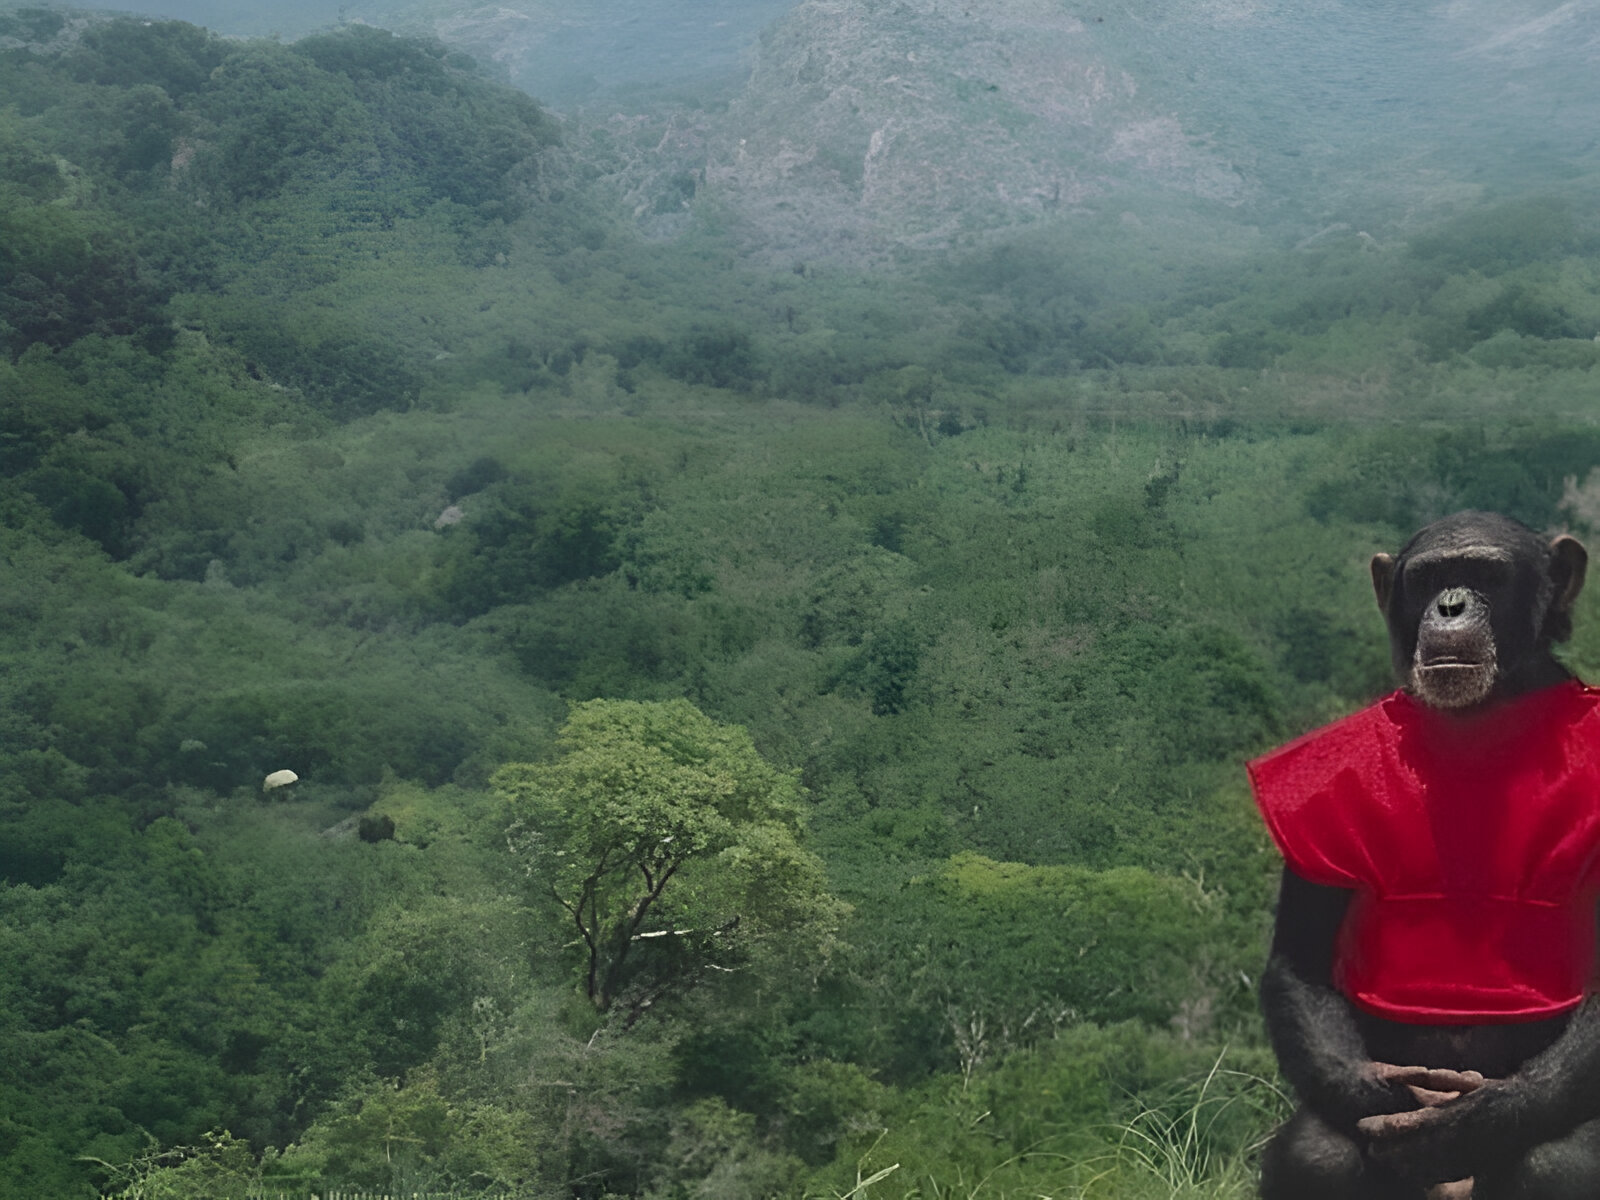
\includegraphics[width=\paperwidth,height=\paperheight]{images/assets/monke}}

\frame{\titlepage}}

%------------------------------------------------------------ 
{\usebackgroundtemplate{
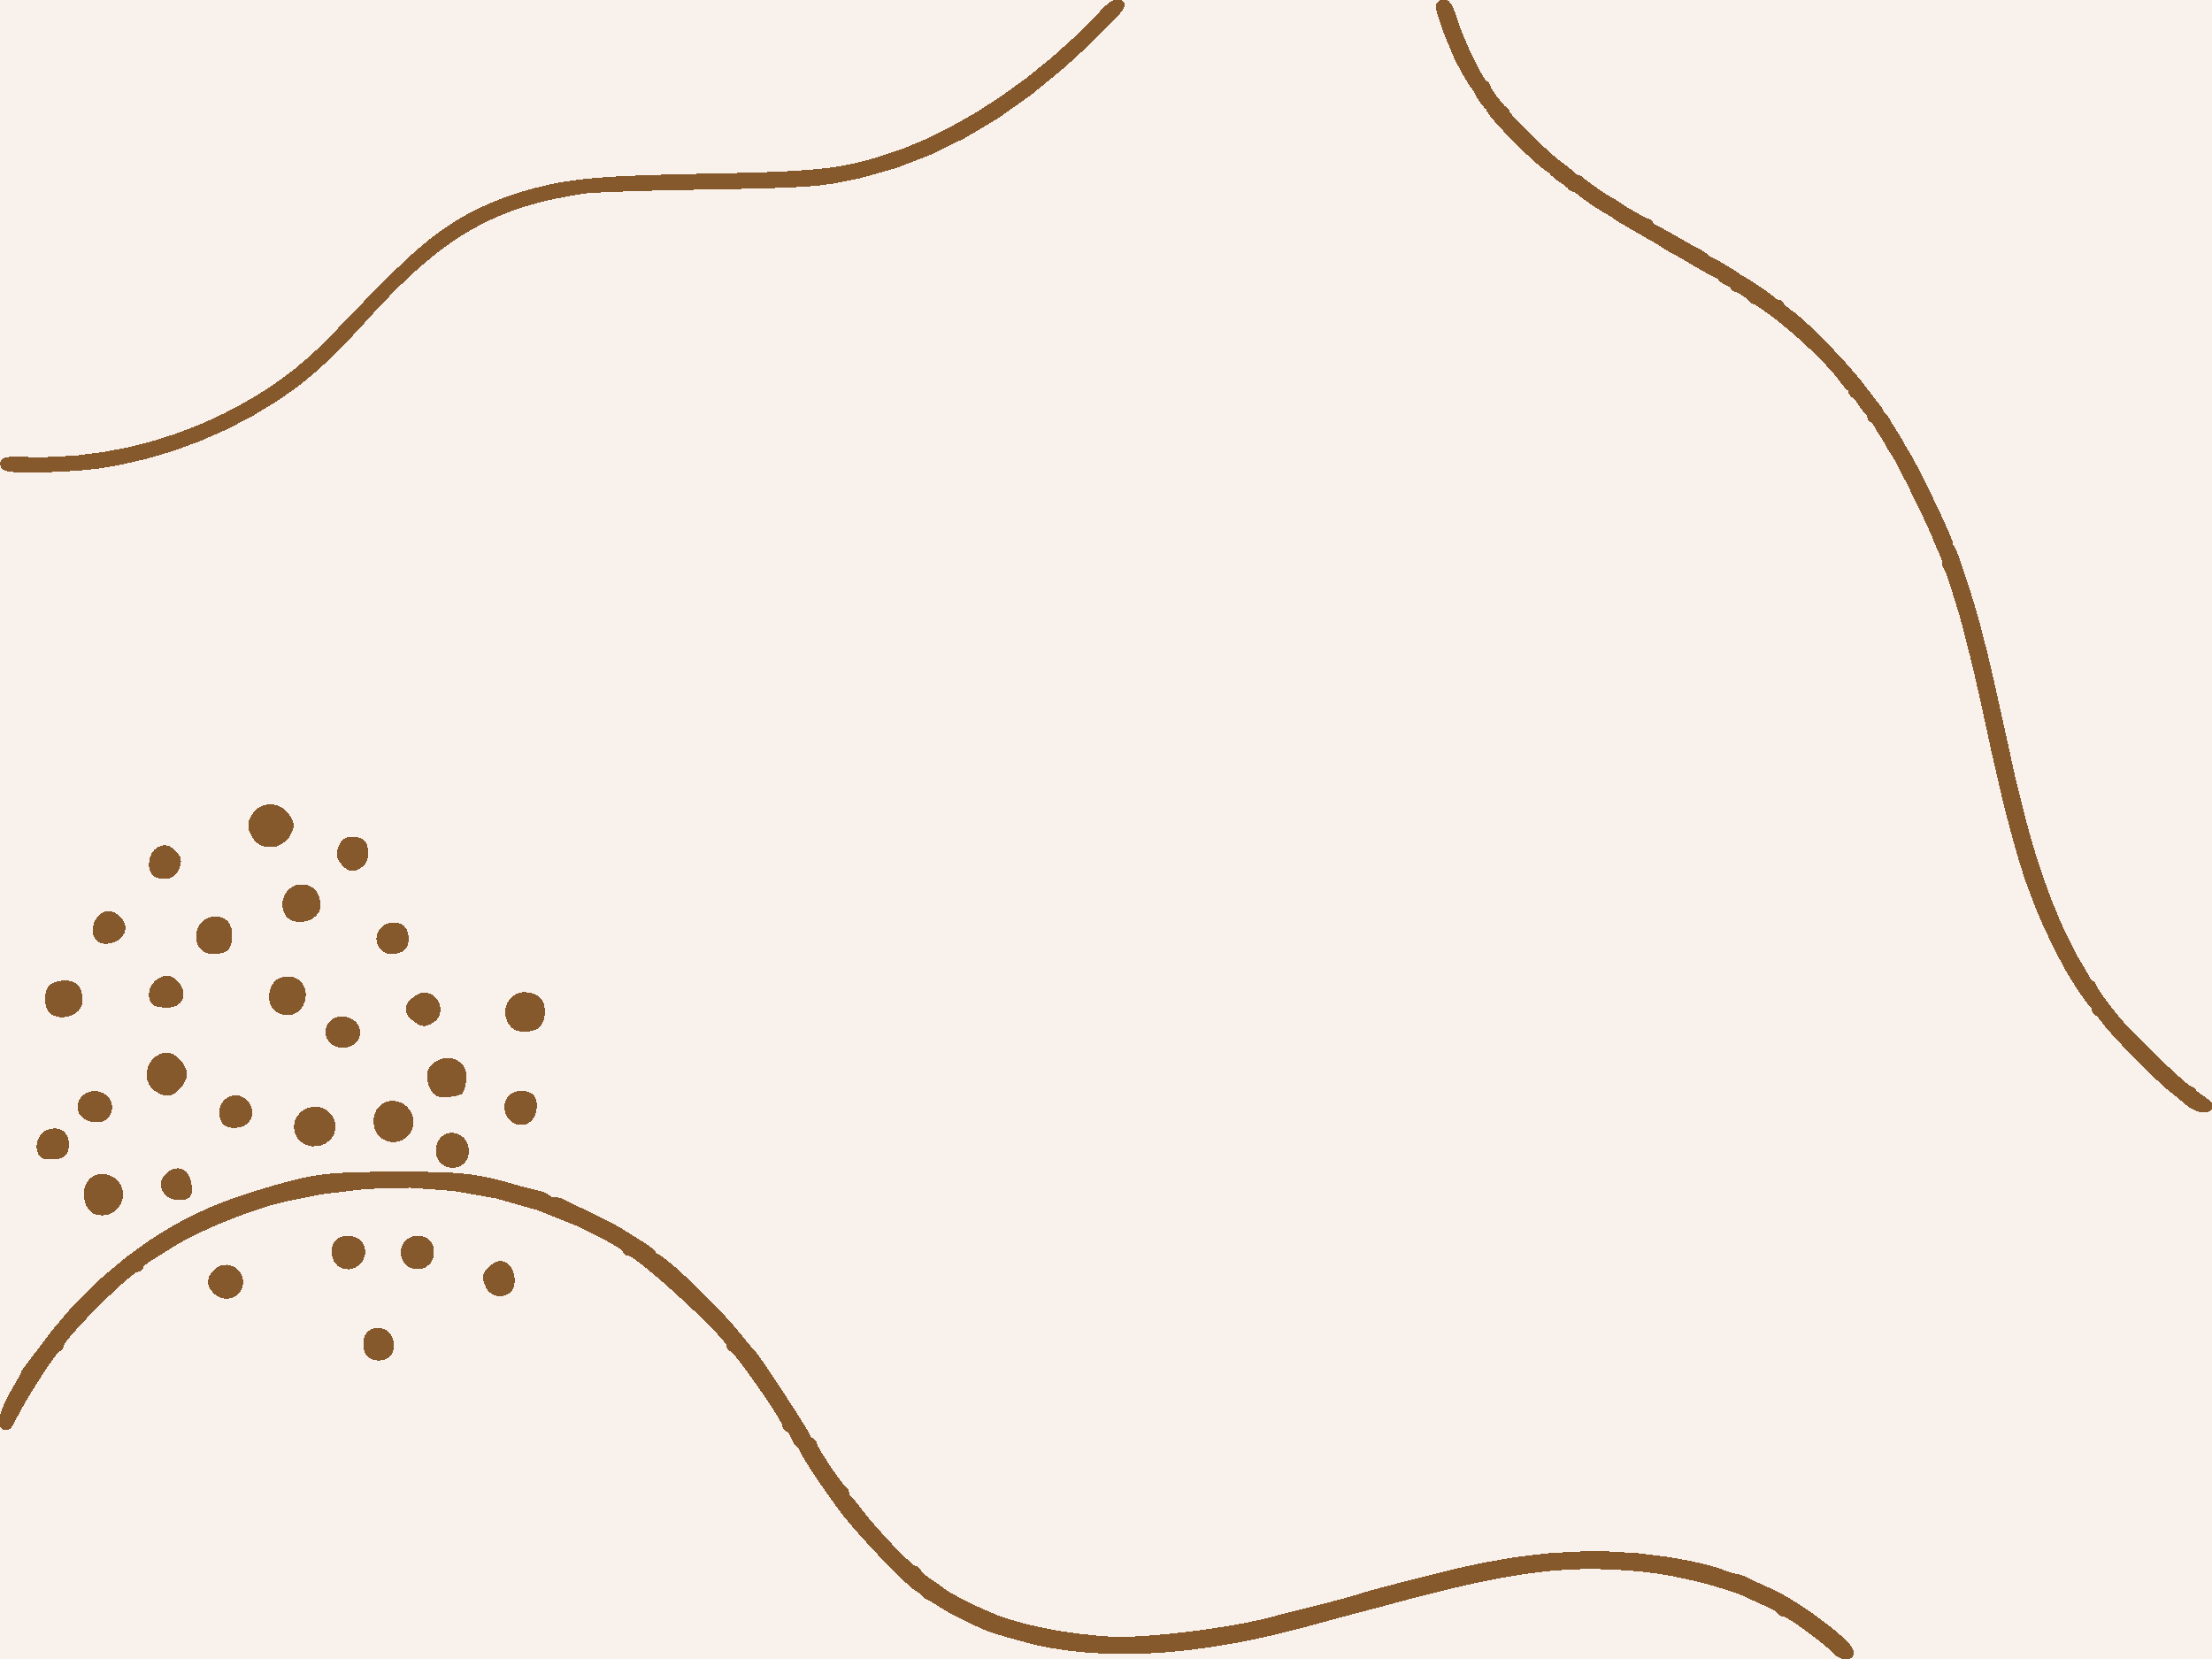
\includegraphics[width=\paperwidth,height=\paperheight]{images/assets/transition}}
\begin{frame}[noframenumbering]

\begin{center}
\Huge \textcolor{brown!70!black}{\textbf{Index}}
\end{center}

\end{frame}}

%------------------------------------------------------------
\begin{frame}{Index}
\pause

\large
\begin{enumerate}
\item Introduction
\item Hartree-Fock-Nambu mean-field theory
\item Lutchyn's miminal Majorana model: 1D SC nanowire of extrinsic homogenous pairing with combined effects of Zeeman and SOC
\pause
\item \textcolor{red!80!black}{\textbf{\underline{Self-consistent nanowires}}} 
\begin{itemize}
\item \textcolor{red!80!black}{Hybrid SC-SM}
\item \textcolor{red!80!black}{Intrinsic}
\end{itemize}
\pause
\item Future works:
\begin{itemize}
\item Josephson junction loop
\item Full-shell Josephson junction
\item Real-time dynamics
\end{itemize}
\end{enumerate}

\end{frame}

%------------------------------------------------------------
{\usebackgroundtemplate{
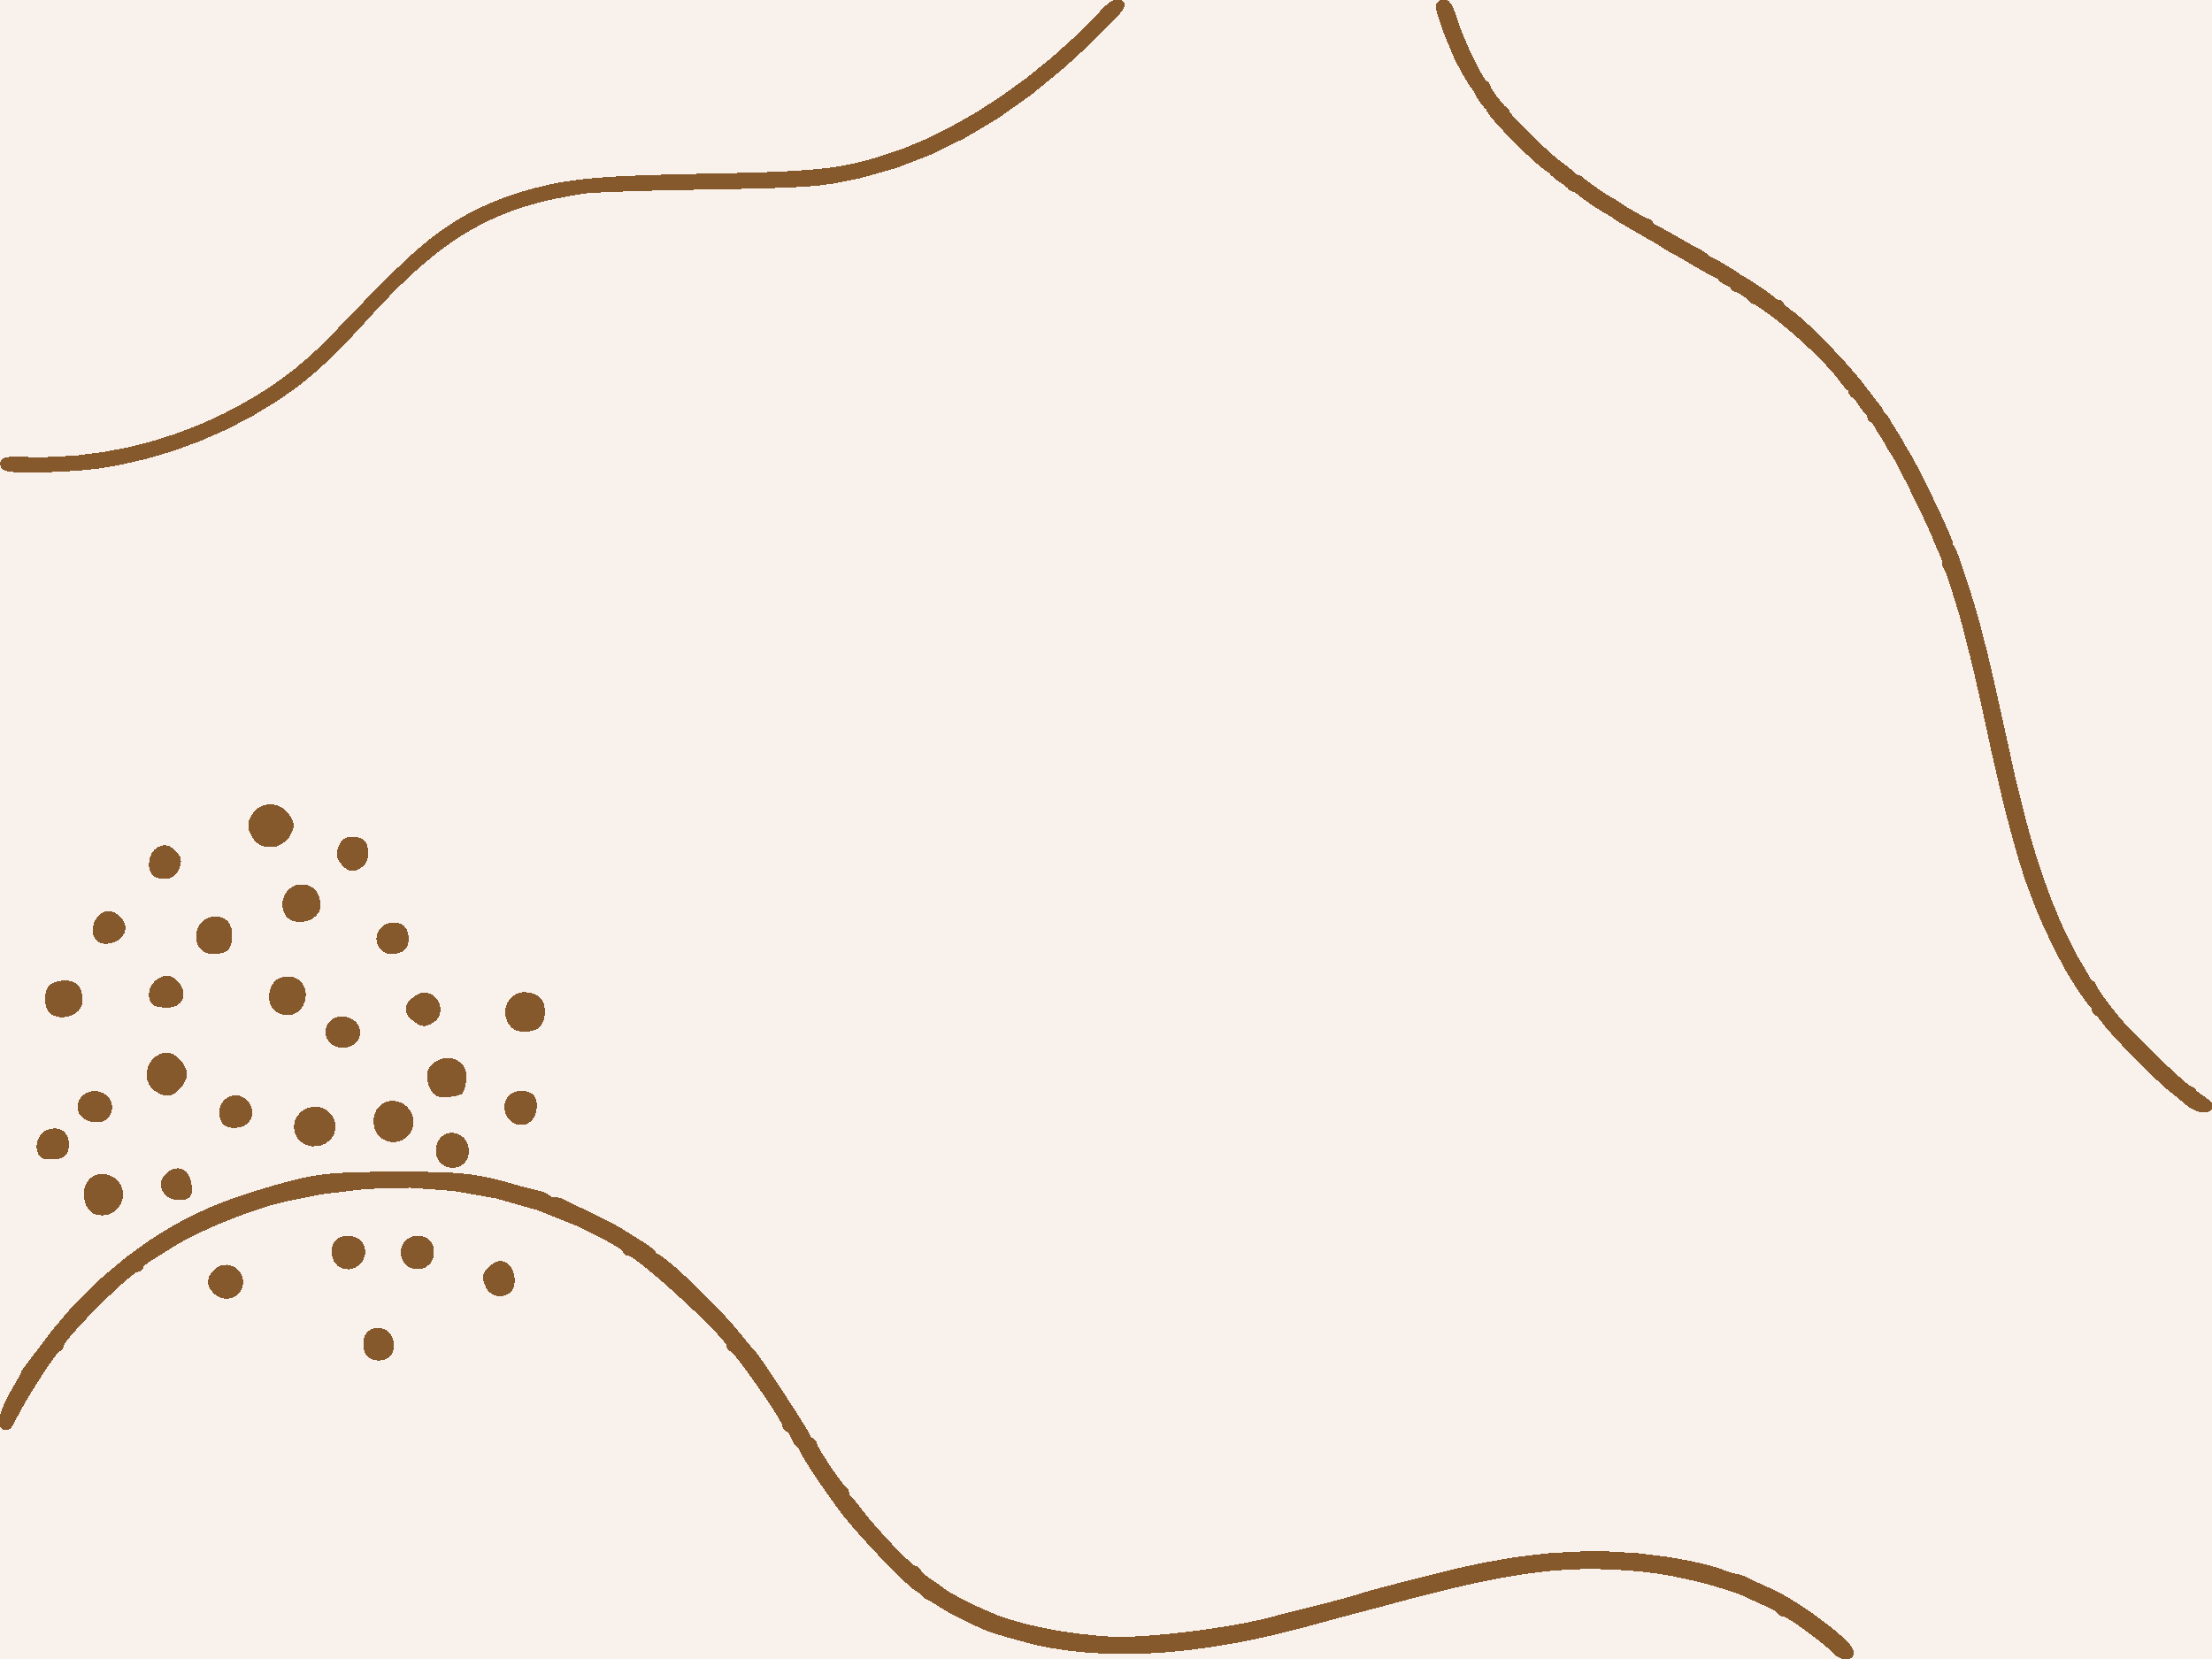
\includegraphics[width=\paperwidth,height=\paperheight]{images/assets/transition}}
\begin{frame}[noframenumbering]

\begin{center}
\Huge \textcolor{brown!70!black}{\textbf{Introduction}}
\end{center}

\end{frame}}

%------------------------------------------------------------
{\setbeamercolor{itemize item}{fg=red!80!black}
\begin{frame}{Introduction}
\pause

\textcolor{red!80!black}{\large \textbf{Landau's Fermi-liquid theory is ideal for normal metals however it fails to describe \underline{superconducting} metals, due to:}}
\begin{itemize}
\item Many-body interactions being "relevant"
\item Large gaps
\item Symmetry breakings
\end{itemize}
\pause

\vspace*{1cm}
\textcolor{red!80!black}{\large \textbf{To study these superconductive systems, we need a \underline{mean-field} theory in order to describe:}}
\begin{itemize}
\item SC ground-states in the presence of magnetic fields
\item Non-intrinsic proximity effects 
\item Time-dependent physics
\end{itemize}

\end{frame}}

%------------------------------------------------------------
{\usebackgroundtemplate{
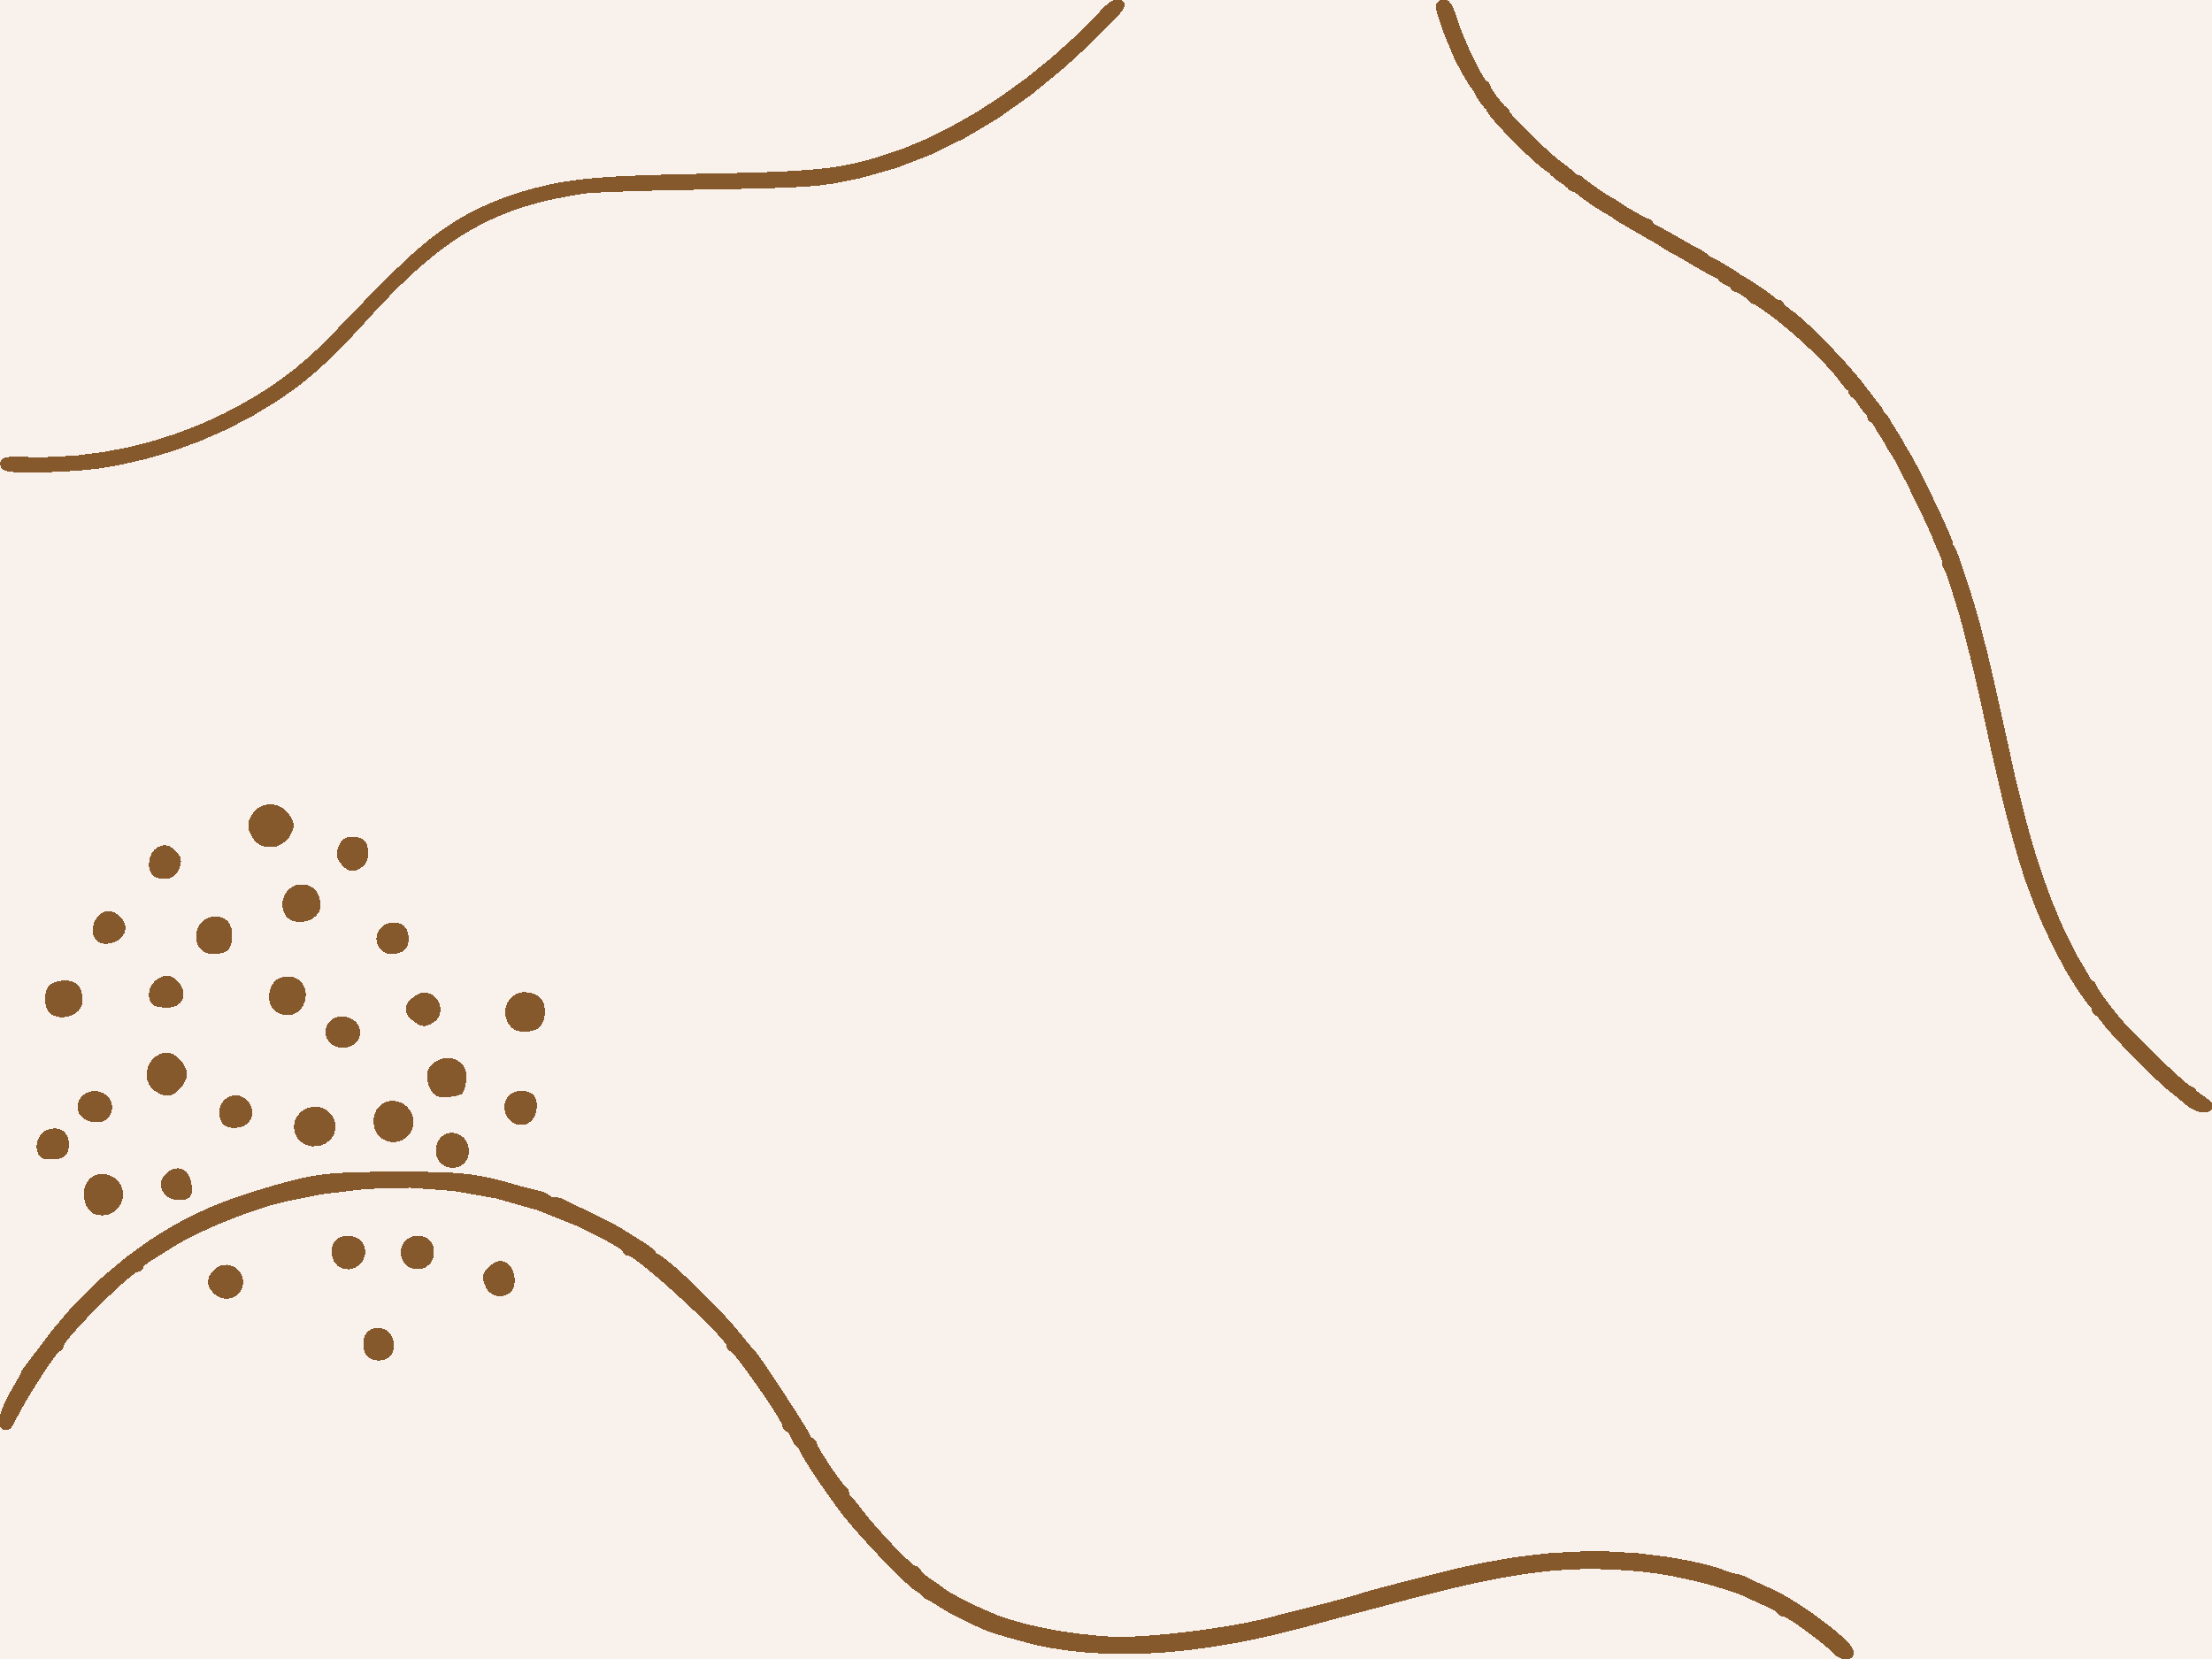
\includegraphics[width=\paperwidth,height=\paperheight]{images/assets/transition}}
\begin{frame}[noframenumbering]

\begin{center}
\Huge \textcolor{brown!70!black}{\textbf{Hartree-Fock-Nambu}} \\
\Huge \textcolor{brown!70!black}{\textbf{mean-field theory}}
\end{center}

\end{frame}}

%------------------------------------------------------------
\begin{frame}
\frametitle{Hartree-Fock-Nambu mean-field theory}

\begin{exampleblock}{Many-body system of electrons}
\begin{equation*}
\hat{H}=\sum_{\alpha\beta}h_{\alpha\beta}c_{\alpha}^{\dagger}c_{\beta}+\frac{1}{2}\sum_{\alpha\beta\gamma\delta}V_{\gamma\delta}^{\alpha\beta}c_{\alpha}^{\dagger}c_{\beta}^{\dagger}c_{\gamma}c_{\delta}
\end{equation*}
\end{exampleblock}
\pause

\begin{columns}
\column{2.5cm}
\begin{alertblock}{Nambu spinor}
\vspace*{-4.5mm}
\begin{equation*}
\check{c}_{a}=\left(\begin{array}{c}
c_{a}\\
c_{a}^{\dagger}
\end{array}\right)
\end{equation*}
\end{alertblock}
\pause

\column{7.5cm}
\begin{exampleblock}{Reduced density matrix (rDM)}
\vspace*{-4.5mm}
\begin{equation*}
\rho_{ab}=\left(\begin{array}{cc}
\langle c_{b}^{\dagger}c_{a}\rangle & \langle c_{b}c_{a}\rangle\\
\langle c_{b}^{\dagger}c_{a}^{\dagger}\rangle & \langle c_{b}c_{a}^{\dagger}\rangle
\end{array}\right)=\left(\begin{array}{cc}
\rho_{ab}^{\text{ee}} & \rho_{ab}^{\text{eh}}\\
\rho_{ab}^{\text{he}} & \rho_{ab}^{\text{hh}}
\end{array}\right)
\end{equation*}
\end{exampleblock}
\pause
\end{columns}

\vspace*{4,5mm}
\begin{itemize} 
\item Solve for the Heinsenberg equation of motion...
\end{itemize}
\pause

\begin{alertblock}{Mean-field decoupling}
\begin{equation*}
\langle c_{\alpha}^{\dagger}c_{\beta}^{\dagger}c_{\gamma}c_{\delta}\rangle\approx\mathfrak{\rho}_{\beta\alpha}^{\text{he}}\mathfrak{\rho}_{\delta\gamma}^{\text{eh}}-\rho_{\gamma\alpha}^{\text{ee}}\rho_{\delta\beta}^{\text{ee}}+\rho_{\delta\alpha}^{\text{ee}}\rho_{\gamma\beta}^{\text{ee}}
\end{equation*}
\end{alertblock}

\end{frame}

%------------------------------------------------------------
\begin{frame}
\frametitle{Hartree-Fock-Nambu mean-field theory}

\begin{exampleblock}{rDM Bogoliubov-de Gennes EoM}
\begin{equation*}
i\hbar\frac{d}{dt}\rho_{ab}=\left[H_{ab}^{\text{BdG}},\rho_{ab}\right]\quad\text{with}\quad H_{\text{BdG}}=\left(\begin{array}{cc}
h_{ab}^{\text{HF}} & \Delta_{ab}\\
\Delta_{ba}^{*} & -h_{ba}^{\text{HF}}
\end{array}\right)
\end{equation*}
\end{exampleblock}
\pause

\begin{columns}
\column{2.5cm}
\begin{center}
\begin{figure}
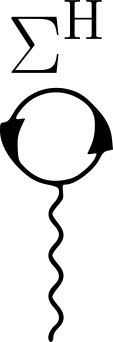
\includegraphics[scale=0.5]{images/H}
\end{figure}
\end{center}

\column{4.5cm}
\begin{alertblock}{\centering{Hartree, Fock and \\pairing self-energies}}
\begin{align*}
\Sigma_{ab}^{H}=&\sum_{\gamma\delta}V_{b\gamma}^{\delta a}\rho_{\gamma\delta}^{\text{ee}}\\\Sigma_{ab}^{F}=&-\sum_{\gamma\delta}V_{b\gamma}^{a\delta}\rho_{\gamma\delta}^{\text{ee}}\\\Delta_{ab}=&\sum_{\gamma\delta}V_{\delta\gamma}^{ab}\rho_{\gamma\delta}^{\text{eh}}
\end{align*}
\end{alertblock}

\column{4cm}
\begin{center}
\begin{figure}
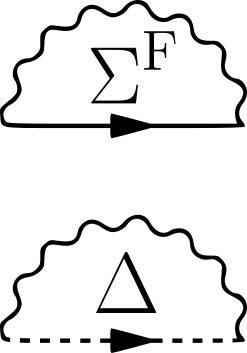
\includegraphics[scale=0.5]{images/FD}
\end{figure}
\end{center}
\end{columns}

\end{frame}

%------------------------------------------------------------
\begin{frame}
\frametitle{Hartree-Fock-Nambu mean-field theory}

\begin{exampleblock}{Tight-binding scheme accounting for spin, $a\rightarrow i\sigma_{i}$}
\begin{equation*}
\boldsymbol{\rho}_{ij}=\left(\begin{array}{cc}
\boldsymbol{\rho}_{ij}^{\text{\text{ee}}} & \boldsymbol{\rho}_{ij}^{\text{eh}}\\
\boldsymbol{\rho}_{ji}^{\text{he}} & \boldsymbol{\rho}_{ji}^{\text{\text{hh}}}
\end{array}\right)=\left(\begin{array}{cc|cc}
\rho_{i\uparrow j\uparrow}^{\text{ee}} & \rho_{i\uparrow j\downarrow}^{\text{ee}} & \rho_{i\uparrow j\uparrow}^{\text{eh}} & \rho_{i\uparrow j\downarrow}^{\text{eh}}\\
\rho_{i\downarrow j\uparrow}^{\text{ee}} & \rho_{i\downarrow j\downarrow}^{\text{ee}} & \rho_{s\downarrow\uparrow}^{\text{eh}} & \rho_{i\downarrow j\downarrow}^{\text{eh}}\\
\hline \rho_{i\uparrow j\uparrow}^{\text{he}} & \rho_{i\uparrow j\downarrow}^{\text{he}} & \rho_{i\uparrow j\uparrow}^{\text{hh}} & \rho_{i\downarrow j\uparrow}^{\text{hh}}\\
\rho_{i\downarrow j\uparrow}^{\text{he}} & \rho_{i\downarrow j\downarrow}^{\text{he}} & \rho_{i\uparrow j\downarrow}^{\text{hh}} & \rho_{i\downarrow j\downarrow}^{\text{hh}}
\end{array}\right)
\end{equation*}
\end{exampleblock}
\pause

\begin{columns}
\column{3cm}
\begin{alertblock}{Wannier limit}
\vspace*{-4mm}
\begin{equation*}
V_{\gamma\delta}^{\alpha\beta}\approx V^{\alpha\beta}\delta_{\alpha\delta}\delta_{\beta\gamma}
\end{equation*}
\end{alertblock}
\begin{alertblock}{Spinless potential}
\vspace*{-4mm}
\begin{equation*}
V^{i\sigma_{i}j\sigma_{j}}=V^{ij}
\end{equation*}
\end{alertblock}
\pause

\column{8cm}
\begin{exampleblock}{Hartree, Fock and Pairing self-energies}
\vspace*{-4mm}
\begin{align*}
\Sigma_{i\sigma_{i}j\sigma_{j}}^{H}=&\sum_{s}V^{is}\left(\rho_{s\uparrow s\uparrow}^{\text{\text{ee}}}+\rho_{s\downarrow s\downarrow}^{\text{\text{ee}}}\right)\delta_{ij}\delta_{\sigma_{i}\sigma_{j}}\\\Sigma_{i\sigma_{i}j\sigma_{j}}^{F}=&-V^{ij}\rho_{i\sigma_{i}j\sigma_{j}}^{\text{ee}}\text{ and }\,\Delta_{i\sigma_{i}j\sigma_{j}}=V^{ij}\rho_{i\sigma_{i}j\sigma_{j}}^{\text{eh}}
\end{align*}
\end{exampleblock}
\end{columns}

\end{frame}

%------------------------------------------------------------
\setbeamercolor*{palette primary}{bg=red!80!black, fg=white}
\setbeamercolor*{palette secondary}{bg=red!80!black, fg=white}
\setbeamercolor*{palette tertiary}{bg=red!80!black, fg=white} 
\begin{frame}
\frametitle{Hartree-Fock-Nambu mean-field theory}

\begin{center}
\Large \textcolor{red!80!black}{$\bigstar$ \textbf{1st objective $\bigstar$}}
\end{center}

\begin{columns}
\column{5cm}

\column{3cm}
\begin{block}{Hubbard limit}
\vspace*{-4mm}
\begin{equation*}
V^{ij}=U\delta_{ij}
\end{equation*}
\end{block}

\column{5cm}
\end{columns}

\begin{block}{\centering{Onsite Hubbard total self-energy}}
\begin{equation*}
\boldsymbol{\Sigma}_{ij}=\frac{1}{2}U\left[\text{Tr}\left(\left[\tau_{z}\otimes\sigma_{0}\right]\tilde{\boldsymbol{\rho}}_{ii}\right)\left[\tau_{z}\otimes\sigma_{0}\right]-2\tilde{\boldsymbol{\rho}}_{ij}\right]\delta_{ij}
\end{equation*}
\end{block}

\begin{columns}
\column{2.5cm}

\column{7cm}
\begin{block}{}
\vspace*{-4.5mm}
\begin{equation*}
\text{with}\quad \tilde{\boldsymbol{\rho}}_{ij}=\left(\begin{array}{cc}
\boldsymbol{\rho}_{ij}^{\text{\text{ee}}} & -\boldsymbol{\rho}_{ij}^{\text{eh}}\\
-\left(\boldsymbol{\rho}_{ji}^{\text{eh}}\right)^{*} & -\boldsymbol{\rho}_{ji}^{\text{\text{ee}}}
\end{array}\right)
\end{equation*}
\end{block}

\column{2.5cm}
\end{columns}

\end{frame}

%------------------------------------------------------------
\setbeamercolor*{palette primary}{bg=brown!70!white, fg=white}
\setbeamercolor*{palette secondary}{bg=brown!70!white, fg=white}
\setbeamercolor*{palette tertiary}{bg=brown!70!white, fg=white}
{\usebackgroundtemplate{
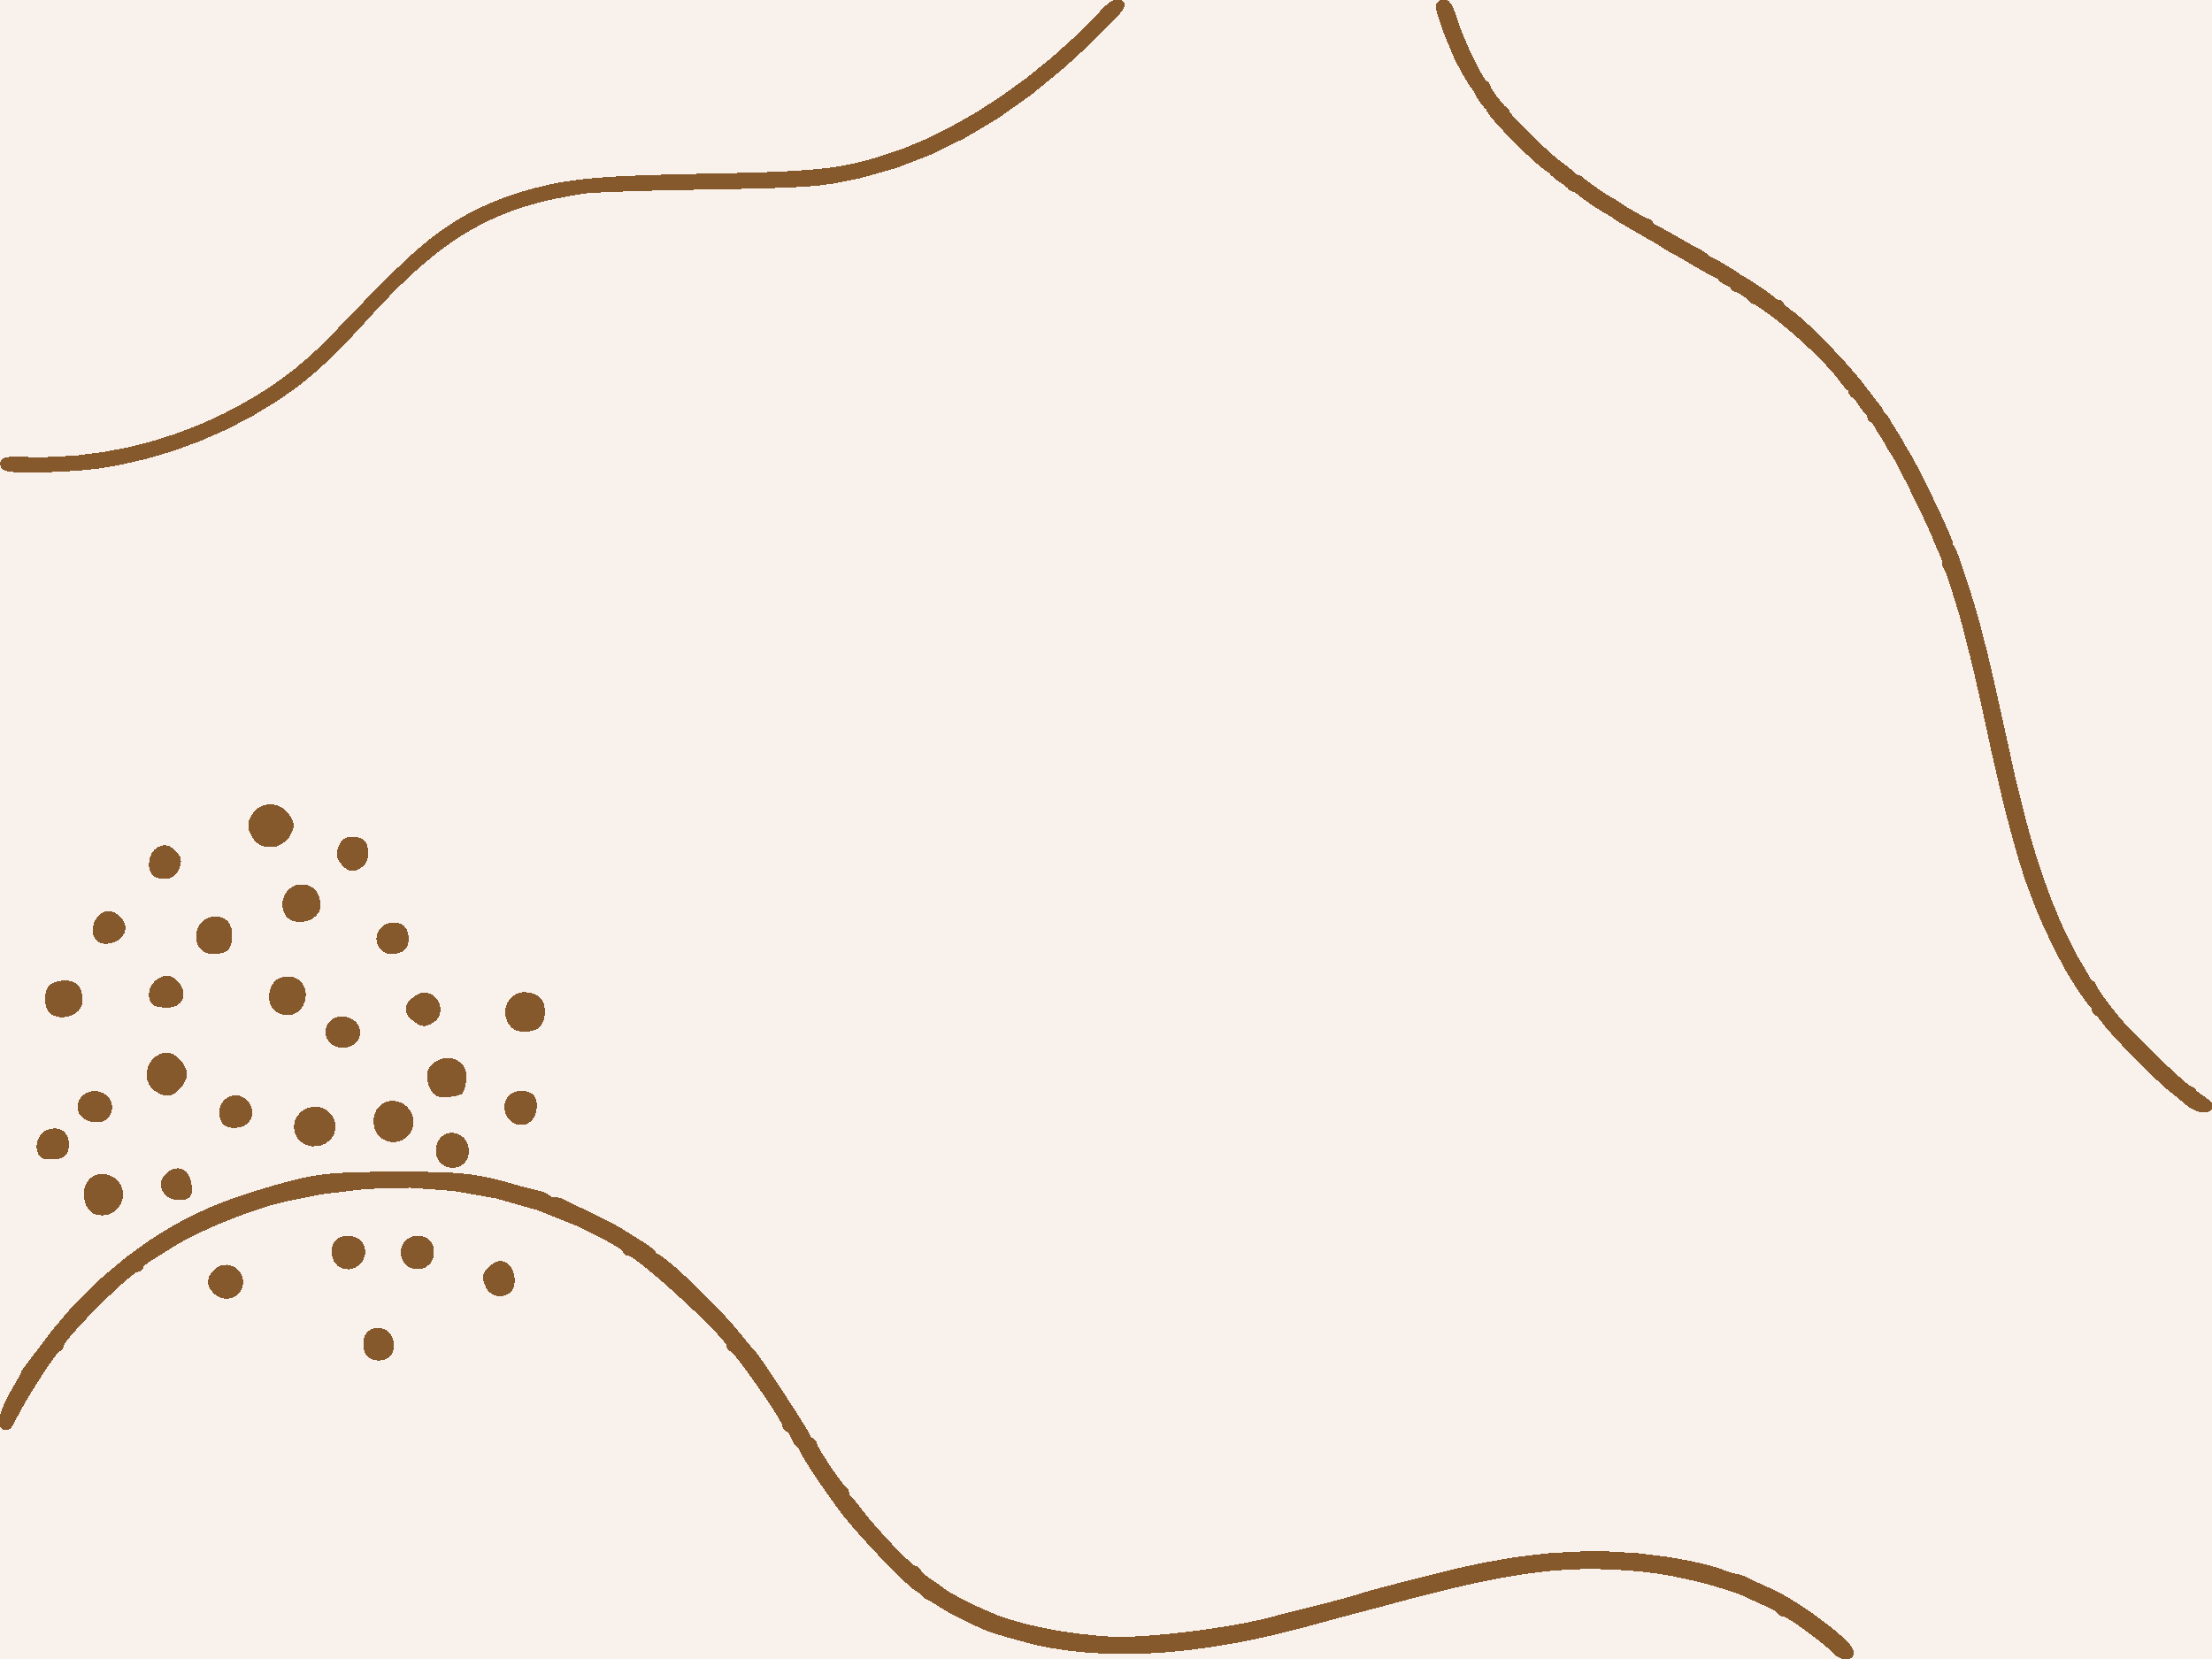
\includegraphics[width=\paperwidth,height=\paperheight]{images/assets/transition}}
\begin{frame}[noframenumbering]

\begin{center}
\Huge \textcolor{brown!70!black}{\textbf{Lutchyn's Mininal}} \\
\Huge \textcolor{brown!70!black}{\textbf{Majorana model}} \\
\end{center}

\end{frame}}

%------------------------------------------------------------
\begin{frame}
\frametitle{Lutchyn's Minimal Majorana model}

\begin{center}
\begin{figure}
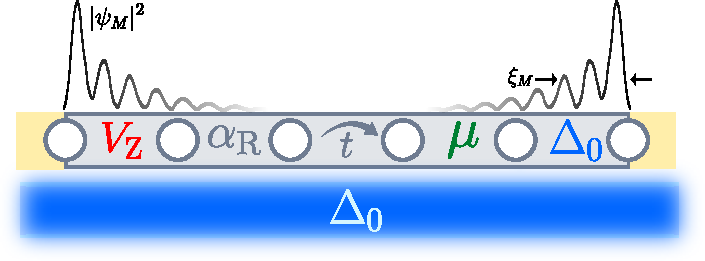
\includegraphics[scale=0.7]{images/model_minimal}
\end{figure}
\end{center}
\vspace*{-5mm}

\begin{columns}
\column{8cm}
\begin{exampleblock}{}
\vspace*{-4.5mm}
\begin{align*}
\boldsymbol{H}_{ij}&=(2t-\mu)\delta_{ij}\left[\tau_{z}\otimes\sigma_{0}\right]\quad\textcolor{ForestGreen!80!black}{\longrightarrow\text{On-site}}\\&\quad-t\delta_{ij\pm1}\left[\tau_{z}\otimes\sigma_{0}\right]\quad\textcolor{ForestGreen!80!black}{\longrightarrow\text{Hoppings}}\\&\quad+\frac{\alpha_{\text{R}}}{2a_{0}}\delta_{ij\pm1}^{\pm}\left[\tau_{z}\otimes i\sigma_{y}\right]\quad\textcolor{ForestGreen!80!black}{\longrightarrow\text{SOC}}\\&\quad+V_{\text{Z}}\left[\tau_{z}\otimes\sigma_{z}\right]\delta_{ij}\quad\textcolor{ForestGreen!80!black}{\longrightarrow\text{Zeeman}}\\&\quad+\Delta_{0}\left[\tau_{y}\otimes\sigma_{y}\right]\delta_{ij}\quad\textcolor{ForestGreen!80!black}{\longrightarrow\text{SC prox.}}
\end{align*}
\end{exampleblock}

\column{3cm}
\begin{alertblock}{Nambu spinor}
\vspace*{-4.5mm}
\begin{equation*}
\boldsymbol{\check{c}}_{i}=\left(\begin{array}{c}
c_{i\uparrow}\\
c_{i\downarrow}\\
c_{i\uparrow}^{\dagger}\\
c_{i\downarrow}^{\dagger}
\end{array}\right)
\end{equation*}
\end{alertblock}
\end{columns}

\begin{exampleblock}{}
\vspace*{-1.5mm}
\begin{equation*}
\text{with:}\quad V_{\text{Z}}=1/2\mu_{B}g_{f}B_{x},\,f=2t-\mu,\,t=\eta/a_{0}^{2},\,\eta=\hbar^{2}/2m^{*}
\end{equation*}
\end{exampleblock}


\end{frame}

%------------------------------------------------------------
\begin{frame}
\frametitle{Lutchyn's Minimal Majorana model}
\pause

\begin{center}
\large \textcolor{red!80!black}{\underline{\textbf{Role of spin-orbit coupling} $\alpha_\text{R}$}}
\end{center}

\begin{center}
\begin{figure}
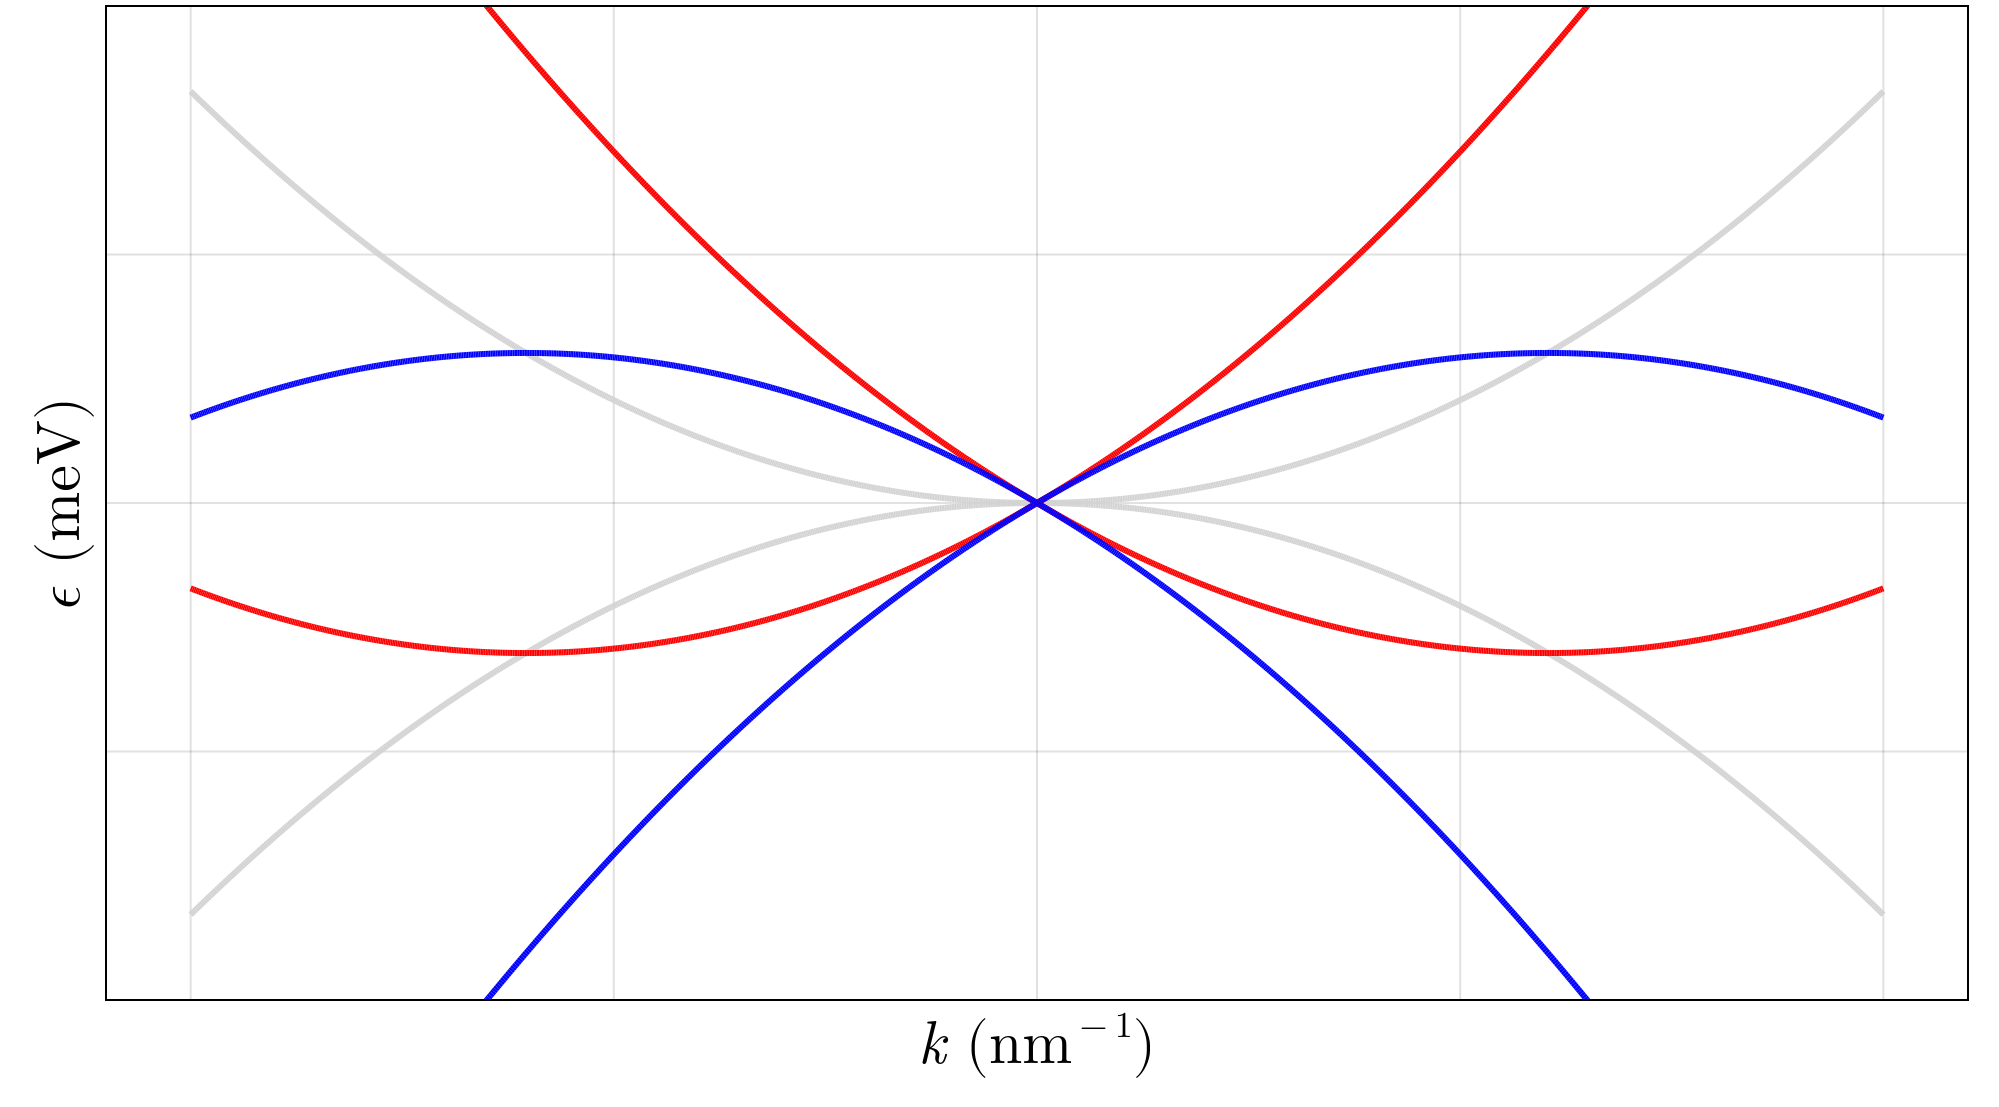
\includegraphics[scale=0.15]{images/lutchyn_bands_SOC}
\end{figure}
\end{center}

\end{frame}

%------------------------------------------------------------
\begin{frame}[noframenumbering]
\frametitle{Lutchyn's Minimal Majorana model}

\begin{center}
\large \textcolor{red!80!black}{\underline{\textbf{Role of chemical potential} $\mu$}}
\end{center}

\begin{center}
\begin{figure}
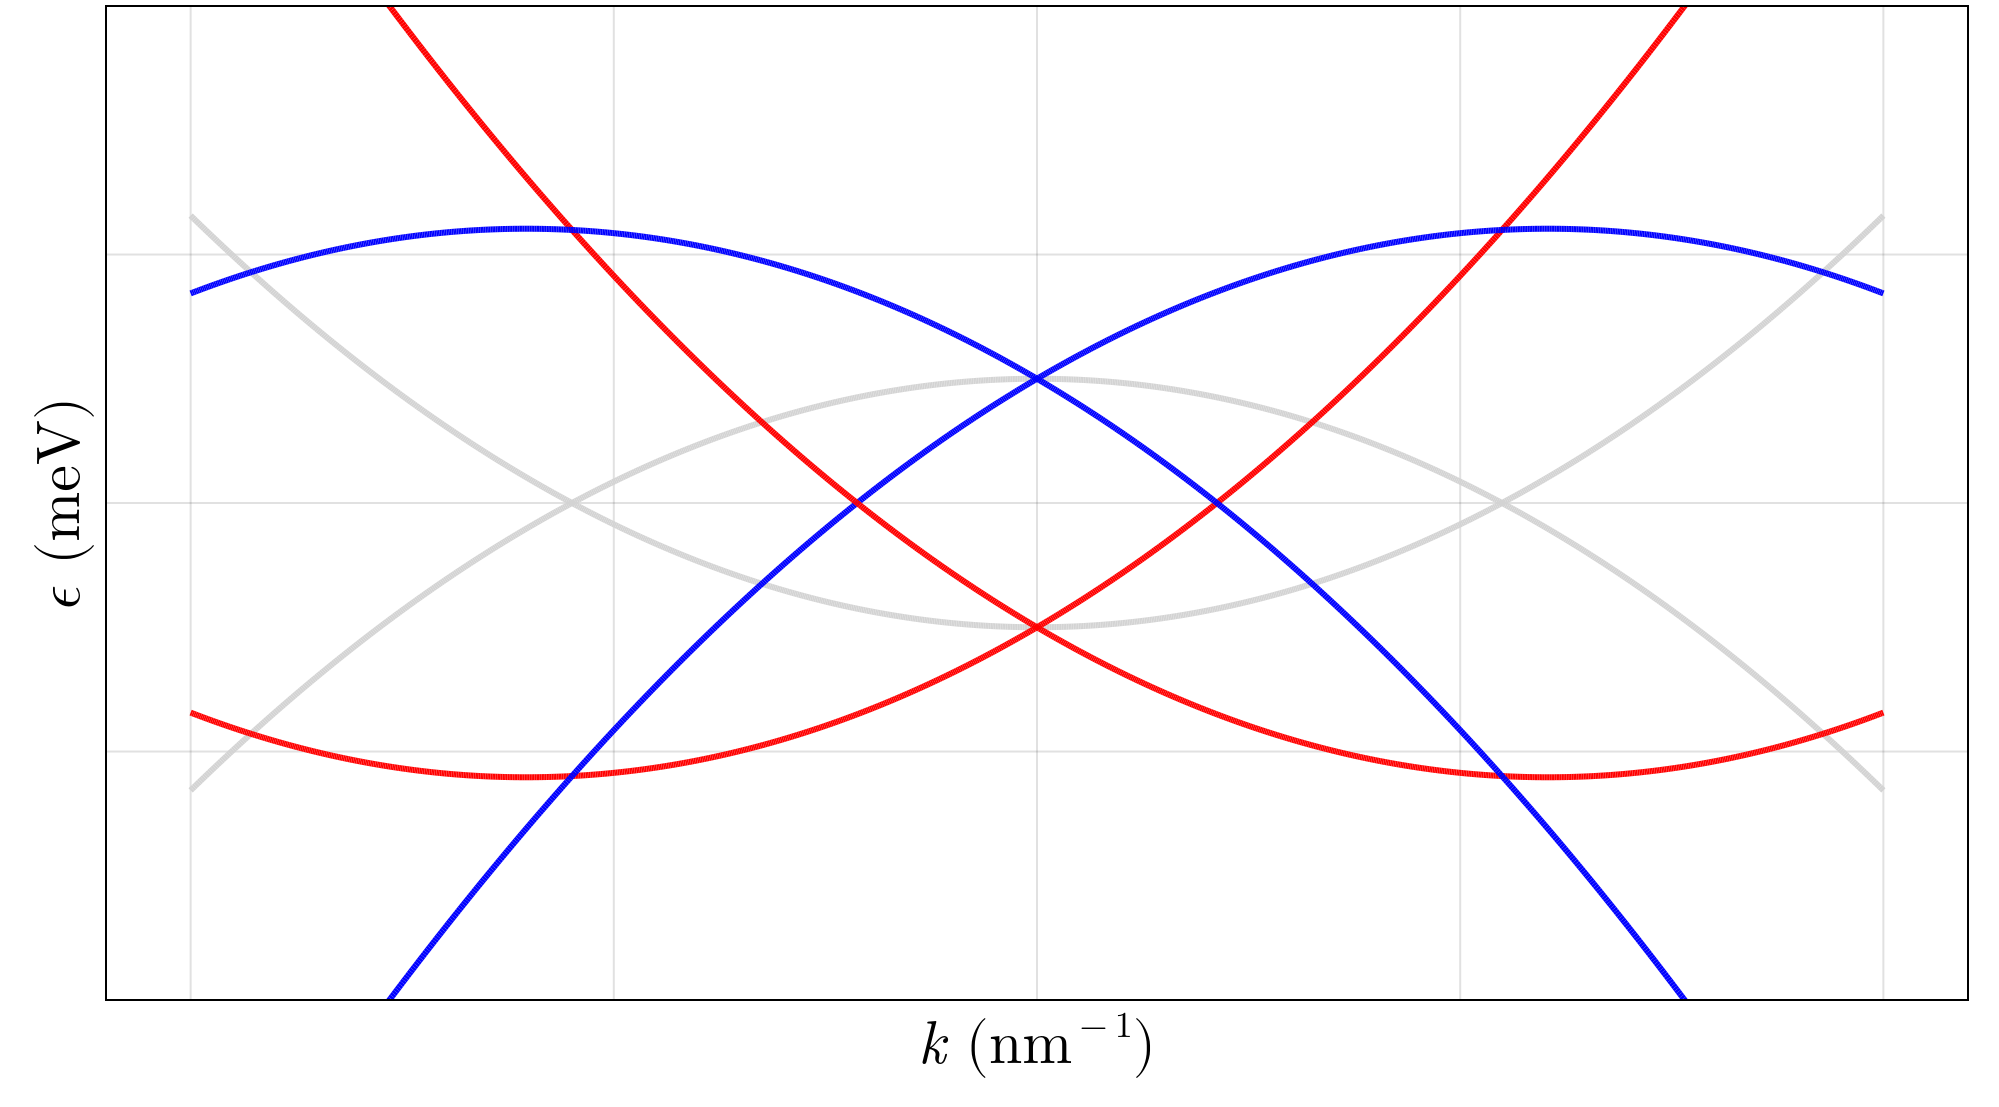
\includegraphics[scale=0.15]{images/lutchyn_bands_chemical}
\end{figure}
\end{center}

\end{frame}

%------------------------------------------------------------
\begin{frame}[noframenumbering]
\frametitle{Lutchyn's Minimal Majorana model}

\begin{center}
\large \textcolor{red!80!black}{\underline{\textbf{Role of Zeeman field} $V_\text{Z}$}}
\end{center}

\begin{center}
\begin{figure}
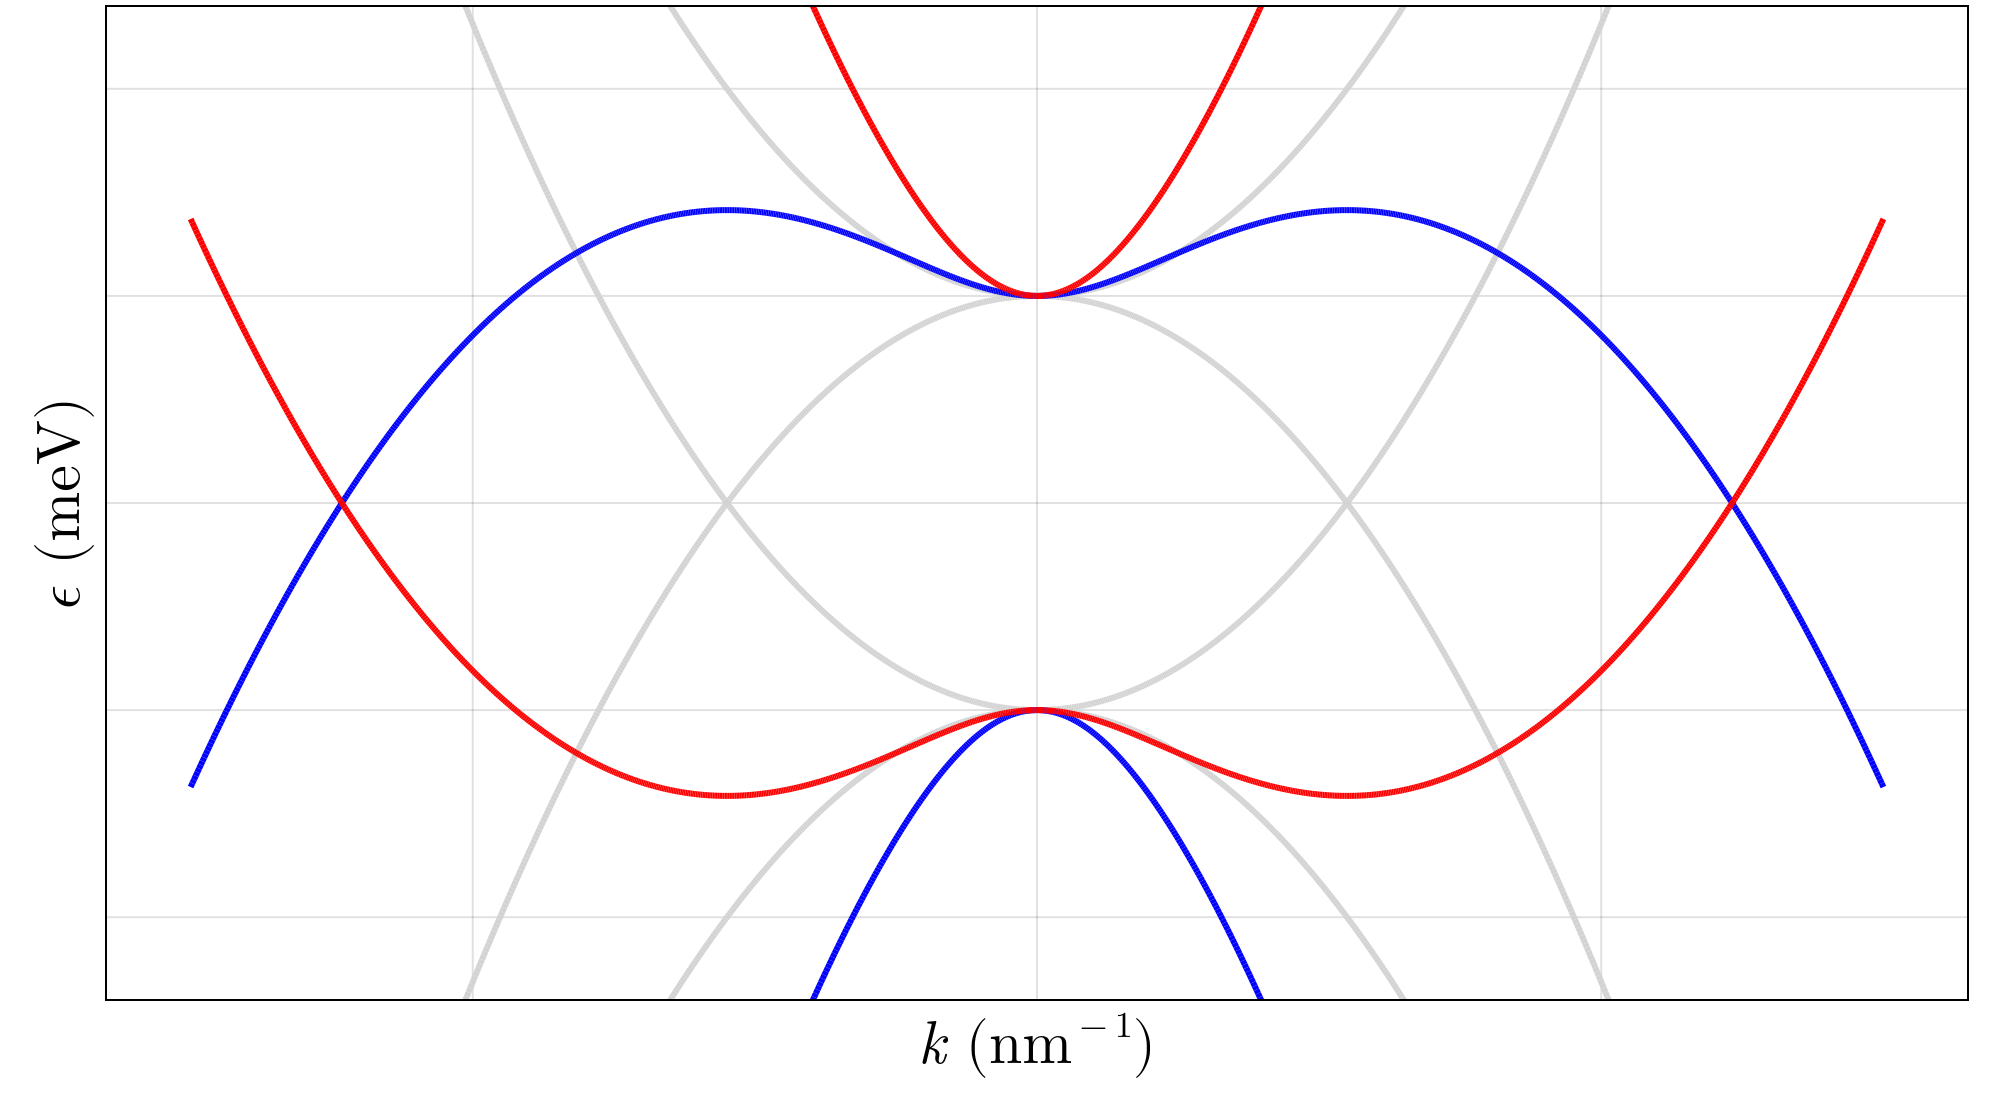
\includegraphics[scale=0.15]{images/lutchyn_bands_zeeman}
\end{figure}
\end{center}

\end{frame}

%------------------------------------------------------------
\begin{frame}[noframenumbering]
\frametitle{Lutchyn's Minimal Majorana model}

\begin{center}
\large \textcolor{red!80!black}{\underline{\textbf{Role of pairing} $\Delta_0$}}
\end{center}

\begin{center}
\begin{figure}
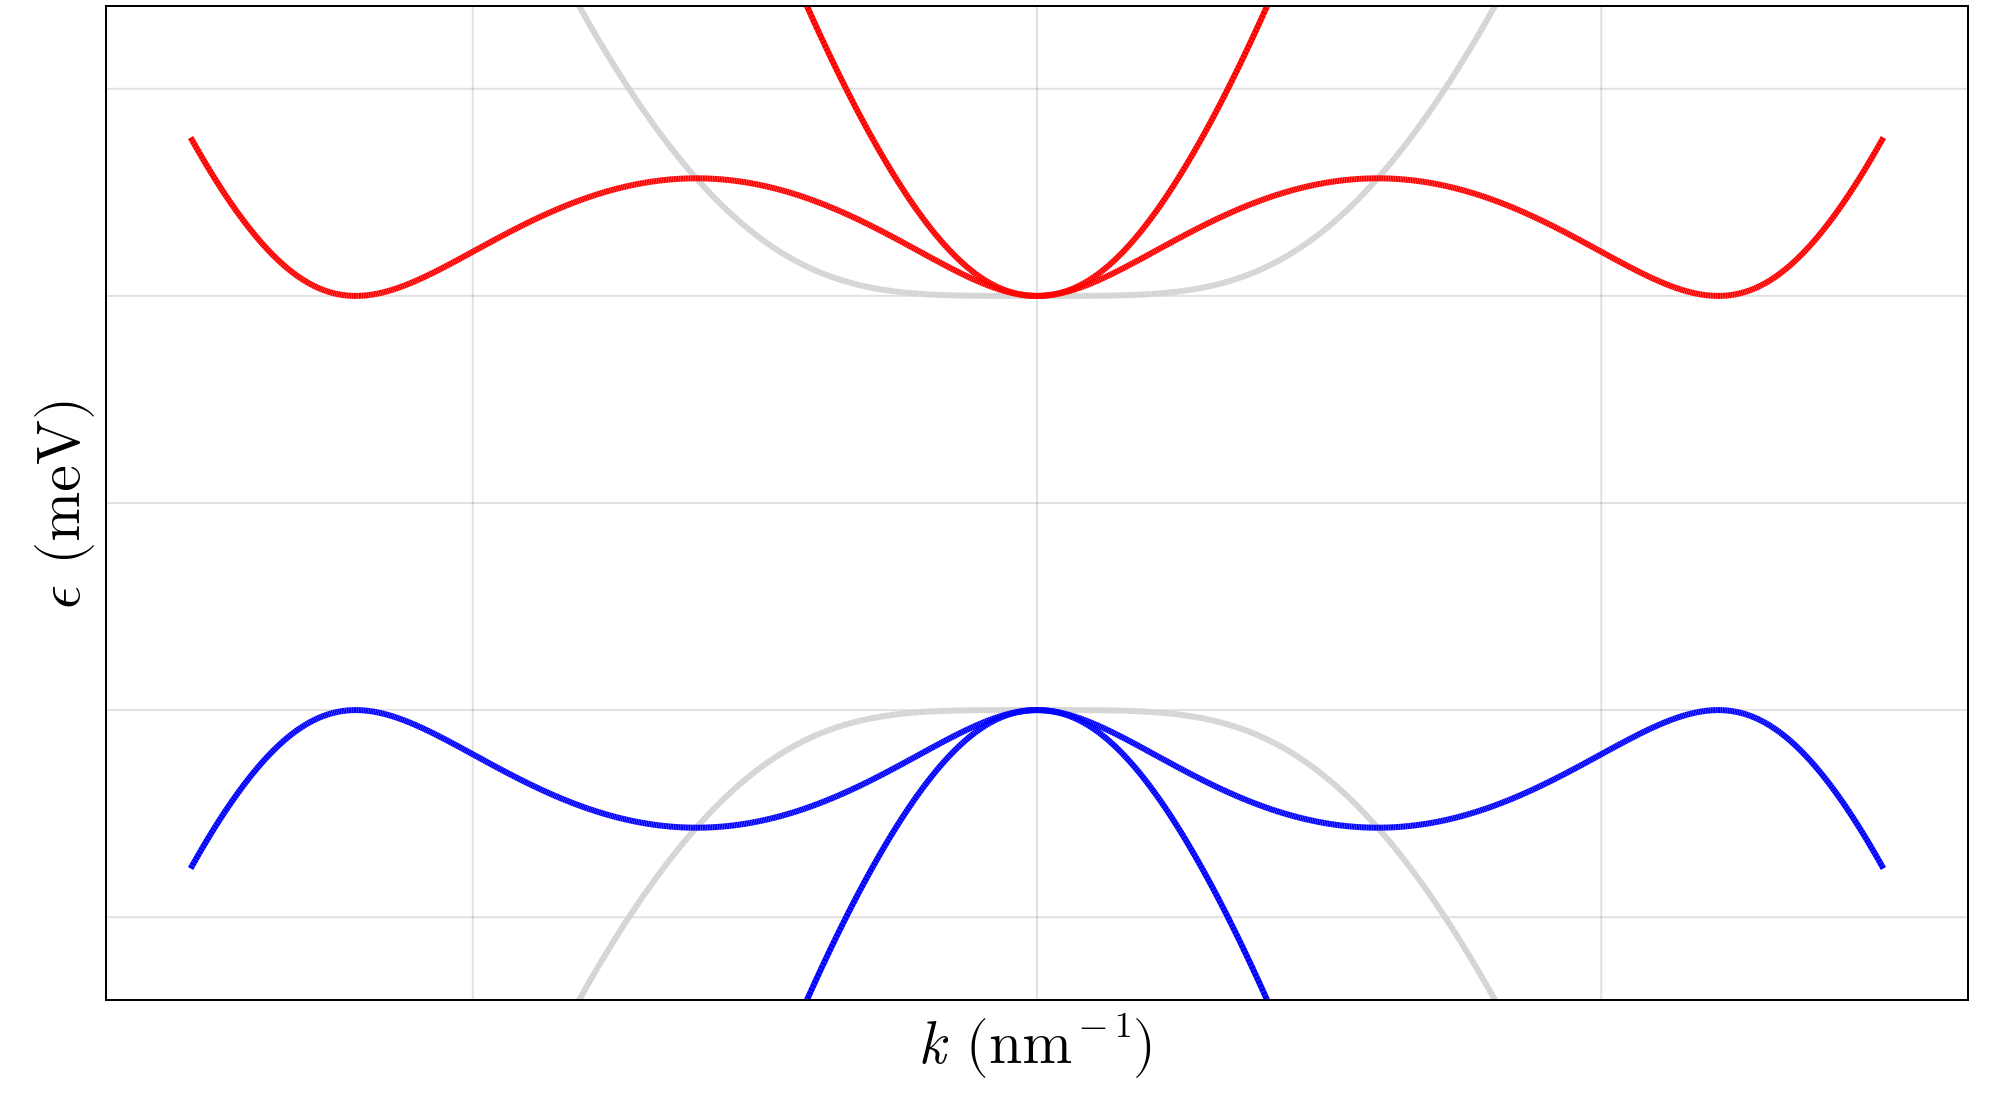
\includegraphics[scale=0.15]{images/lutchyn_bands_pairing}
\end{figure}
\end{center}

\end{frame}

%------------------------------------------------------------
\begin{frame}[noframenumbering]
\frametitle{Lutchyn's Minimal Majorana model}

\begin{center}
\Large \textcolor{red!80!black}{\underline{\textbf{Trivial regime}}}
\end{center}

\begin{center}
\begin{figure}

\includegraphics[scale=0.15]{images/lutchyn_bands_trivial}
\end{figure}
\end{center}

\end{frame}

%------------------------------------------------------------
\begin{frame}[noframenumbering]
\frametitle{Lutchyn's Minimal Majorana model}

\begin{center}
\Large \textcolor{red!80!black}{\underline{\textbf{Critical regime}}}
\end{center}

\begin{center}
\begin{figure}

\includegraphics[scale=0.15]{images/lutchyn_bands_critical}
\end{figure}
\end{center}

\end{frame}

%------------------------------------------------------------
\begin{frame}[noframenumbering]
\frametitle{Lutchyn's Minimal Majorana model}

\begin{center}
\Large \textcolor{red!80!black}{\underline{\textbf{Topological regime}}}
\end{center}

\begin{center}
\begin{figure}

\includegraphics[scale=0.15]{images/lutchyn_bands_topological}
\end{figure}
\end{center}

\end{frame}

%------------------------------------------------------------
\begin{frame}
\frametitle{Lutchyn's Minimal Majorana model}
\pause

\begin{center}
\begin{figure}
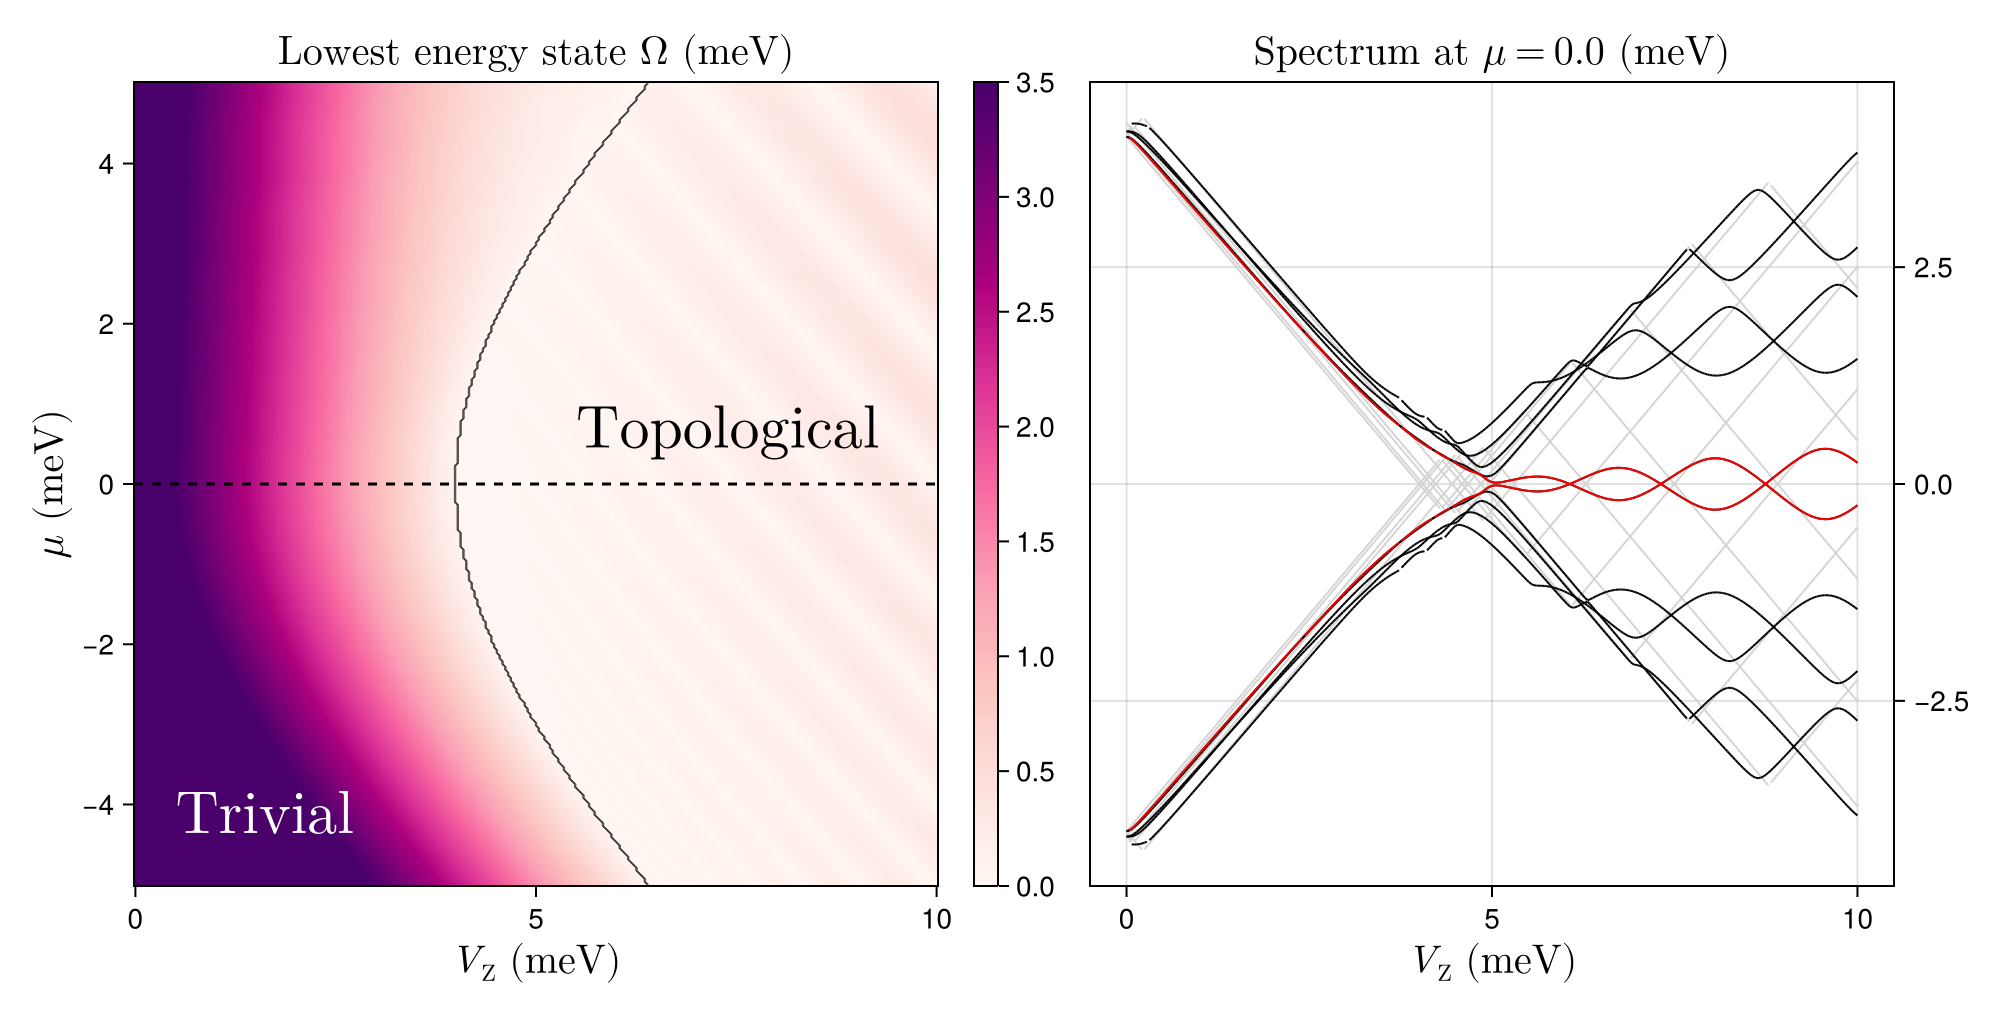
\includegraphics[scale=0.175]{images/lutchyn_majoranas}
\end{figure}
\end{center}

\end{frame}

%------------------------------------------------------------
{\usebackgroundtemplate{
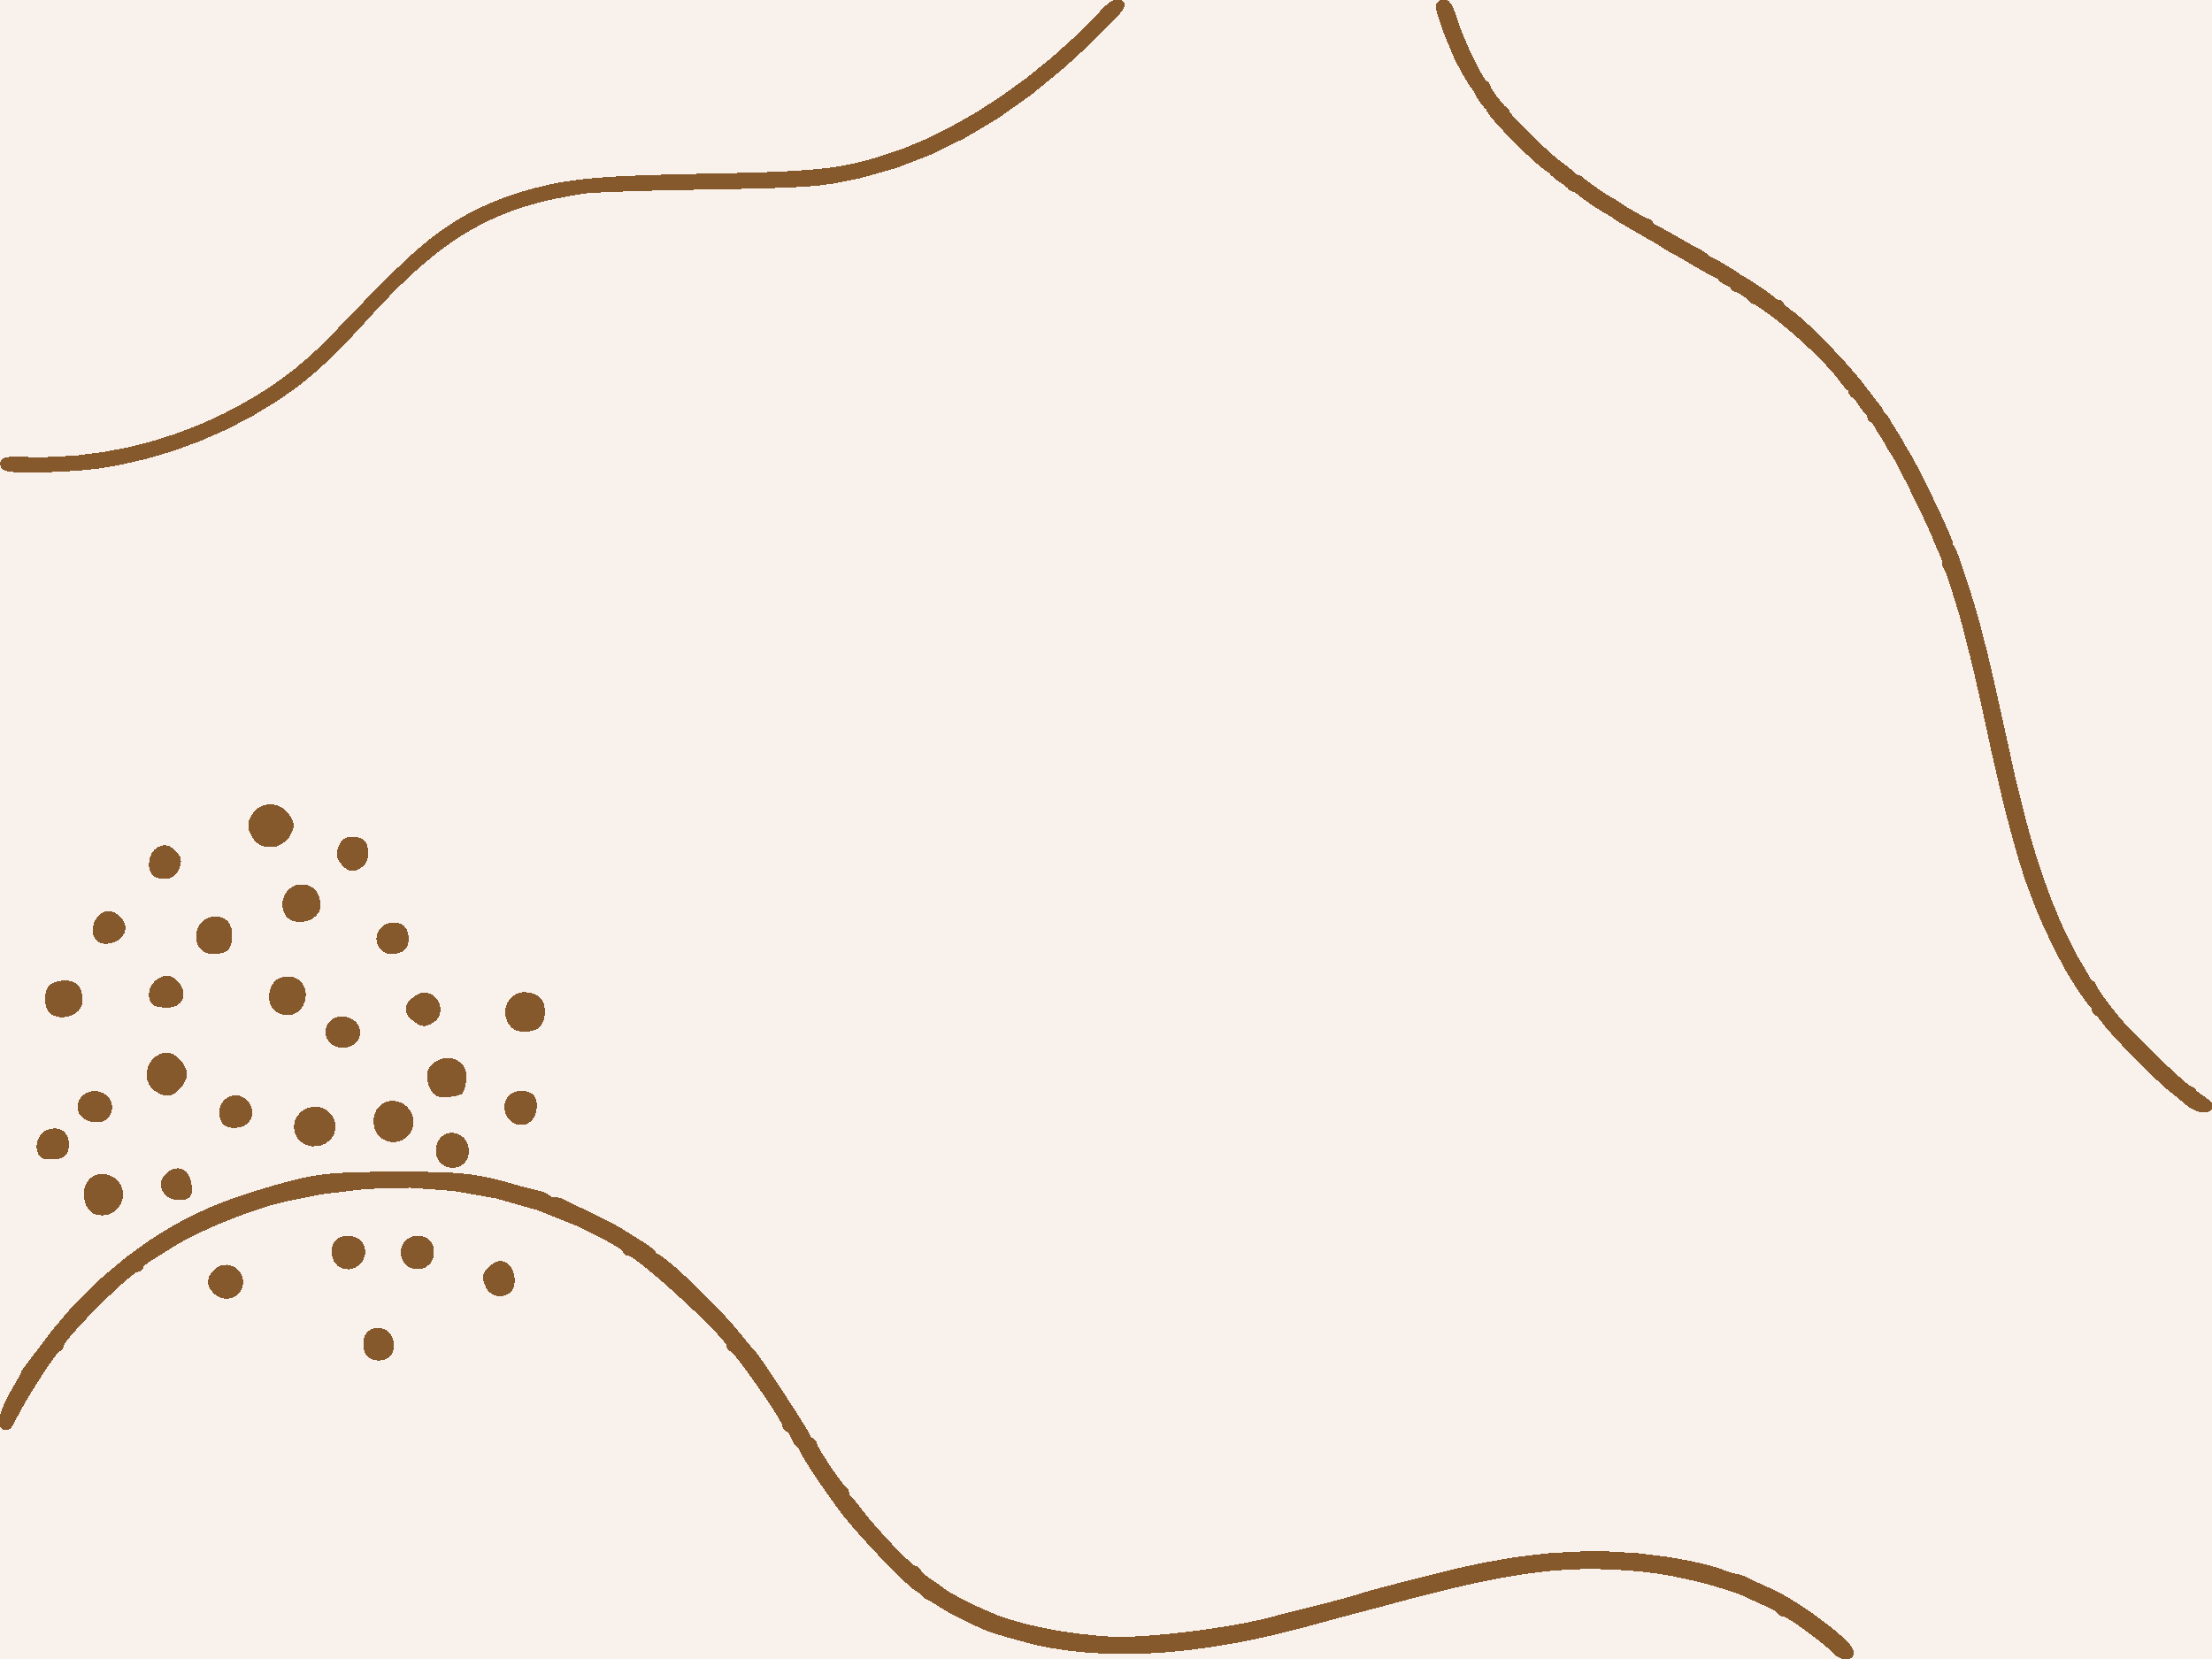
\includegraphics[width=\paperwidth,height=\paperheight]{images/assets/transition}}
\begin{frame}[noframenumbering]

\begin{center}
\Huge \textcolor{brown!70!black}{\textbf{Self-consistent}} \\
\Huge \textcolor{brown!70!black}{\textbf{nanowires}}
\end{center}

\end{frame}}

%------------------------------------------------------------
\begin{frame}
\frametitle{Self-consistent nanowire}

\begin{block}{\centering{Onsite self-energy $\Sigma_{ij}$ instead of homogenous pairing $\Delta_0$}}
\begin{equation*}
\Delta_{0}\left[\tau_{y}\otimes\sigma_{y}\right]\delta_{ij}\,\textcolor{red!80!black}{\longrightarrow}\,U\left(\frac{1}{2}\text{Tr}\left(\left[\tau_{z}\otimes\sigma_{0}\right]\tilde{\boldsymbol{\rho}}_{ii}\right)\left[\tau_{z}\otimes\sigma_{0}\right]-\tilde{\boldsymbol{\rho}}_{ij}\right)\delta_{ij}
\end{equation*}
\end{block}
\pause

\begin{center}
\begin{figure}
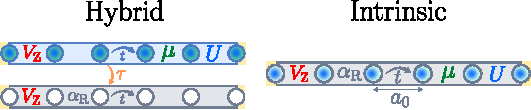
\includegraphics[scale=1.3]{images/model_hybrid_intrinsic}
\end{figure}
\end{center}

\end{frame}

%------------------------------------------------------------
\begin{frame}
\frametitle{\underline{Hybrid} self-consistent nanowire}
\pause

\vspace*{-2mm}
\begin{center}
\begin{figure}
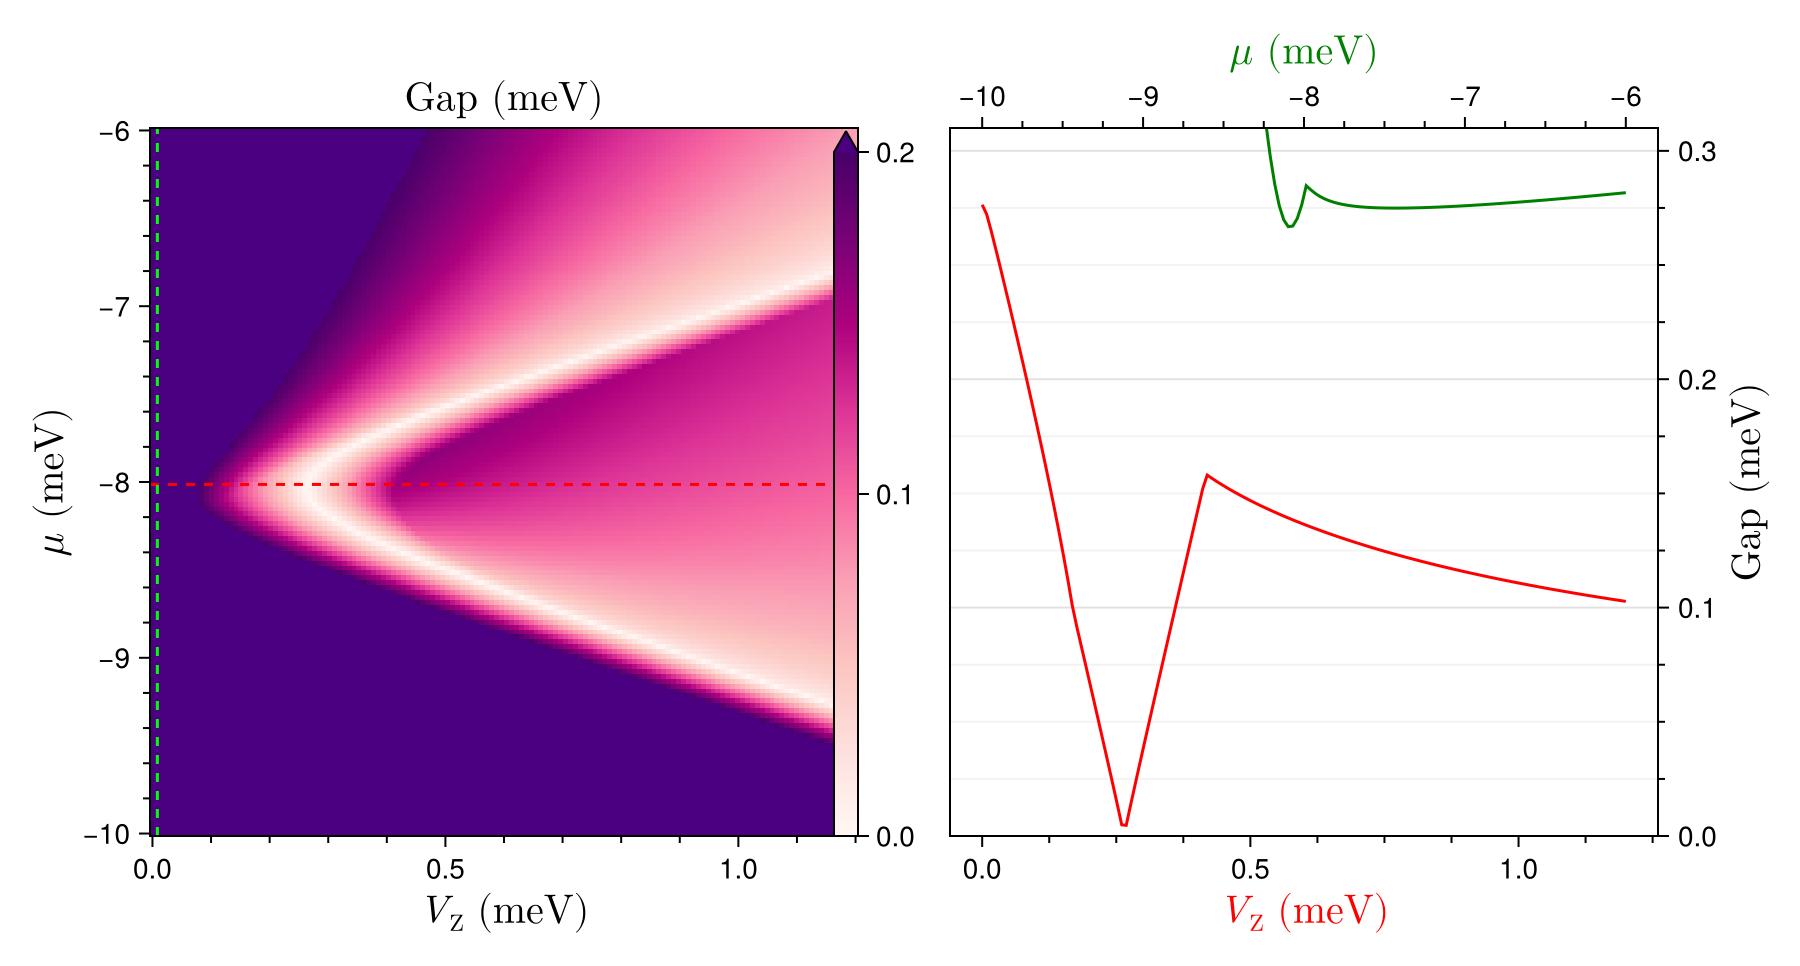
\includegraphics[scale=0.19]{images/hybrid}
\end{figure}
\end{center}

\end{frame}

%------------------------------------------------------------
\setbeamercolor*{palette primary}{bg=red!80!black, fg=white}
\setbeamercolor*{palette secondary}{bg=red!80!black, fg=white}
\setbeamercolor*{palette tertiary}{bg=red!80!black, fg=white}
\begin{frame}
\frametitle{\underline{Intrinsic} self-consistent nanowire}

\begin{columns}
\column{1cm}
\begin{center}
\Large \rotatebox{90}{\textcolor{red!80!black}{$\bigstar$ \textbf{2nd objective $\bigstar$}}}
\end{center}

\column{10cm}
\vspace*{-4mm}
\begin{center}
\begin{figure}
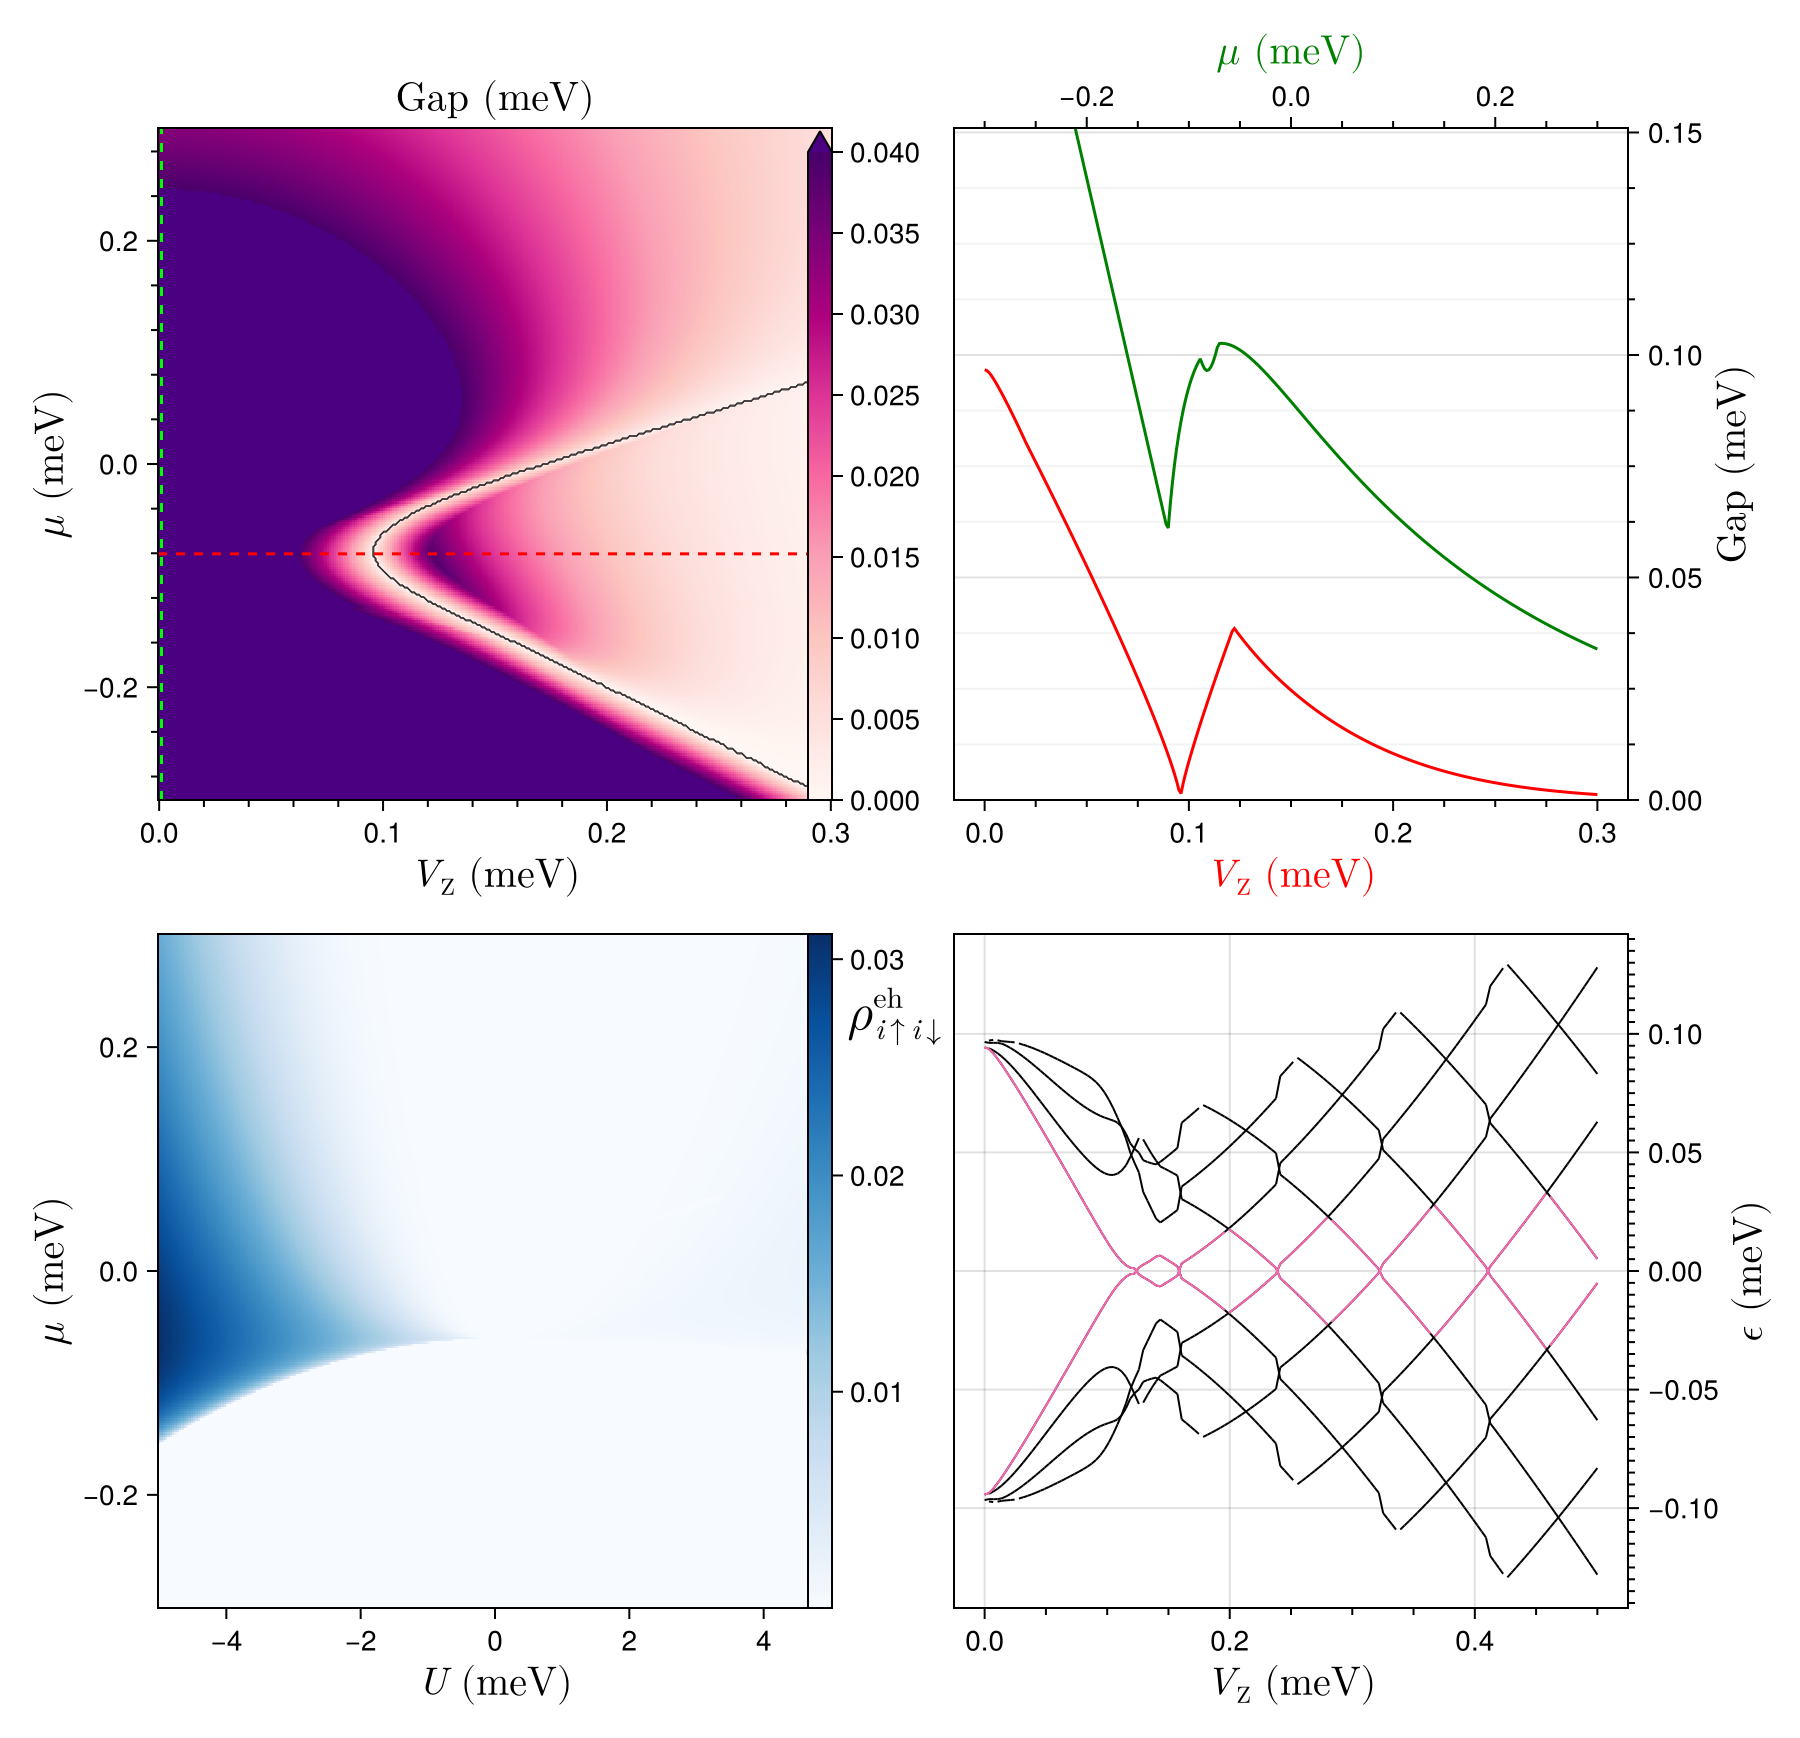
\includegraphics[scale=0.13]{images/intrinsic}
\end{figure}
\end{center}

\column{1cm}
\begin{center}
\Large \rotatebox{90}{\textcolor{red!80!black}{$\dagger$ \textbf{Fails} $\dagger$}}
\end{center}
\end{columns}

\end{frame}

%------------------------------------------------------------
\setbeamercolor*{palette primary}{bg=brown!70!white, fg=white}
\setbeamercolor*{palette secondary}{bg=brown!70!white, fg=white}
\setbeamercolor*{palette tertiary}{bg=brown!70!white, fg=white}
\begin{frame}
\frametitle{\underline{Intrinsic} self-consistent infinite nanowire}

\begin{center}
\begin{figure}
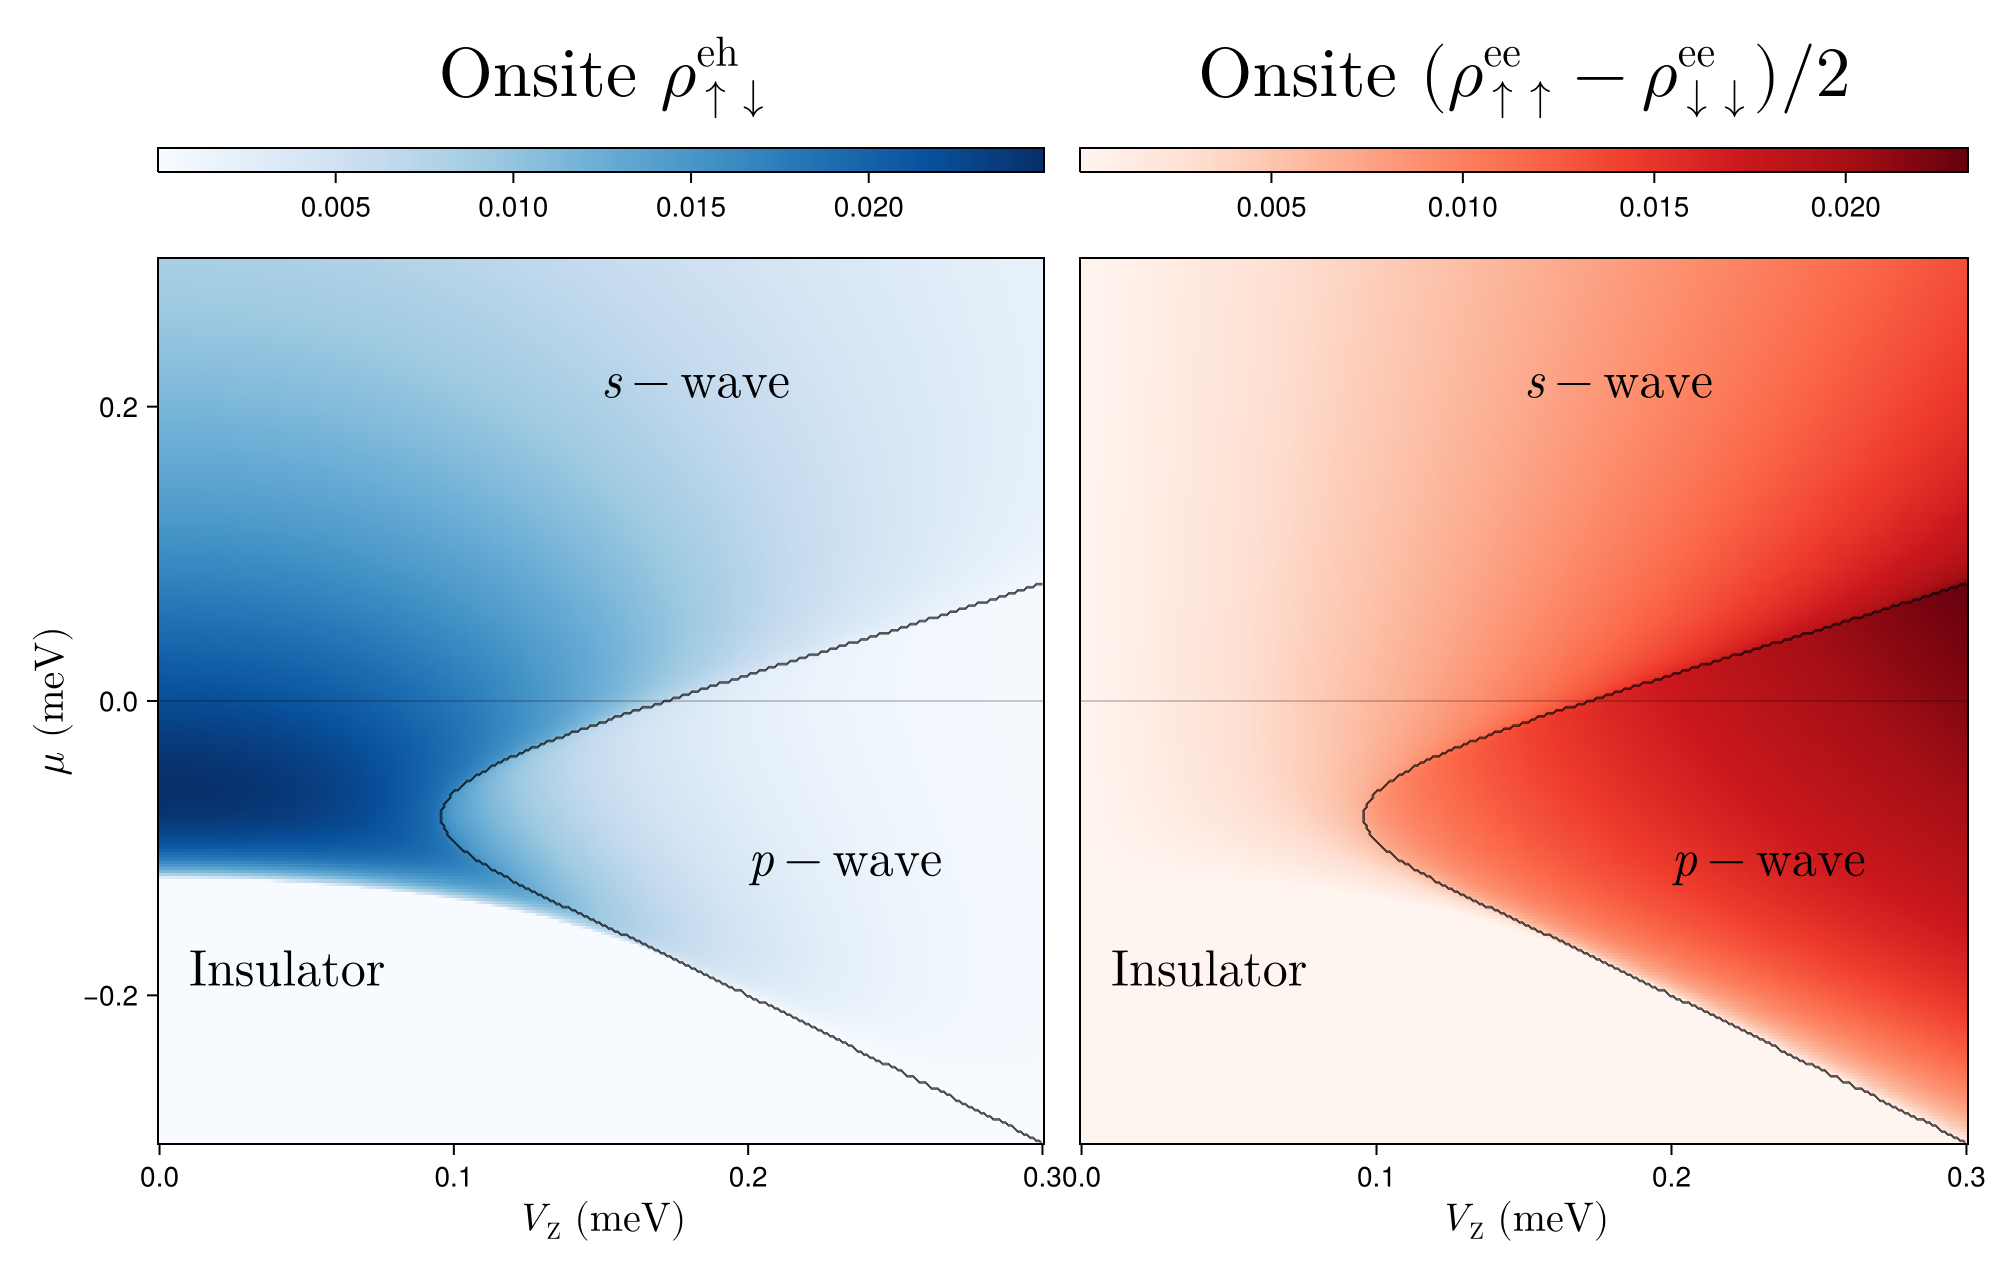
\includegraphics[scale=0.15]{images/intrinsic_infinite_MD}
\end{figure}
\end{center}

\end{frame}

%------------------------------------------------------------
{\usebackgroundtemplate{
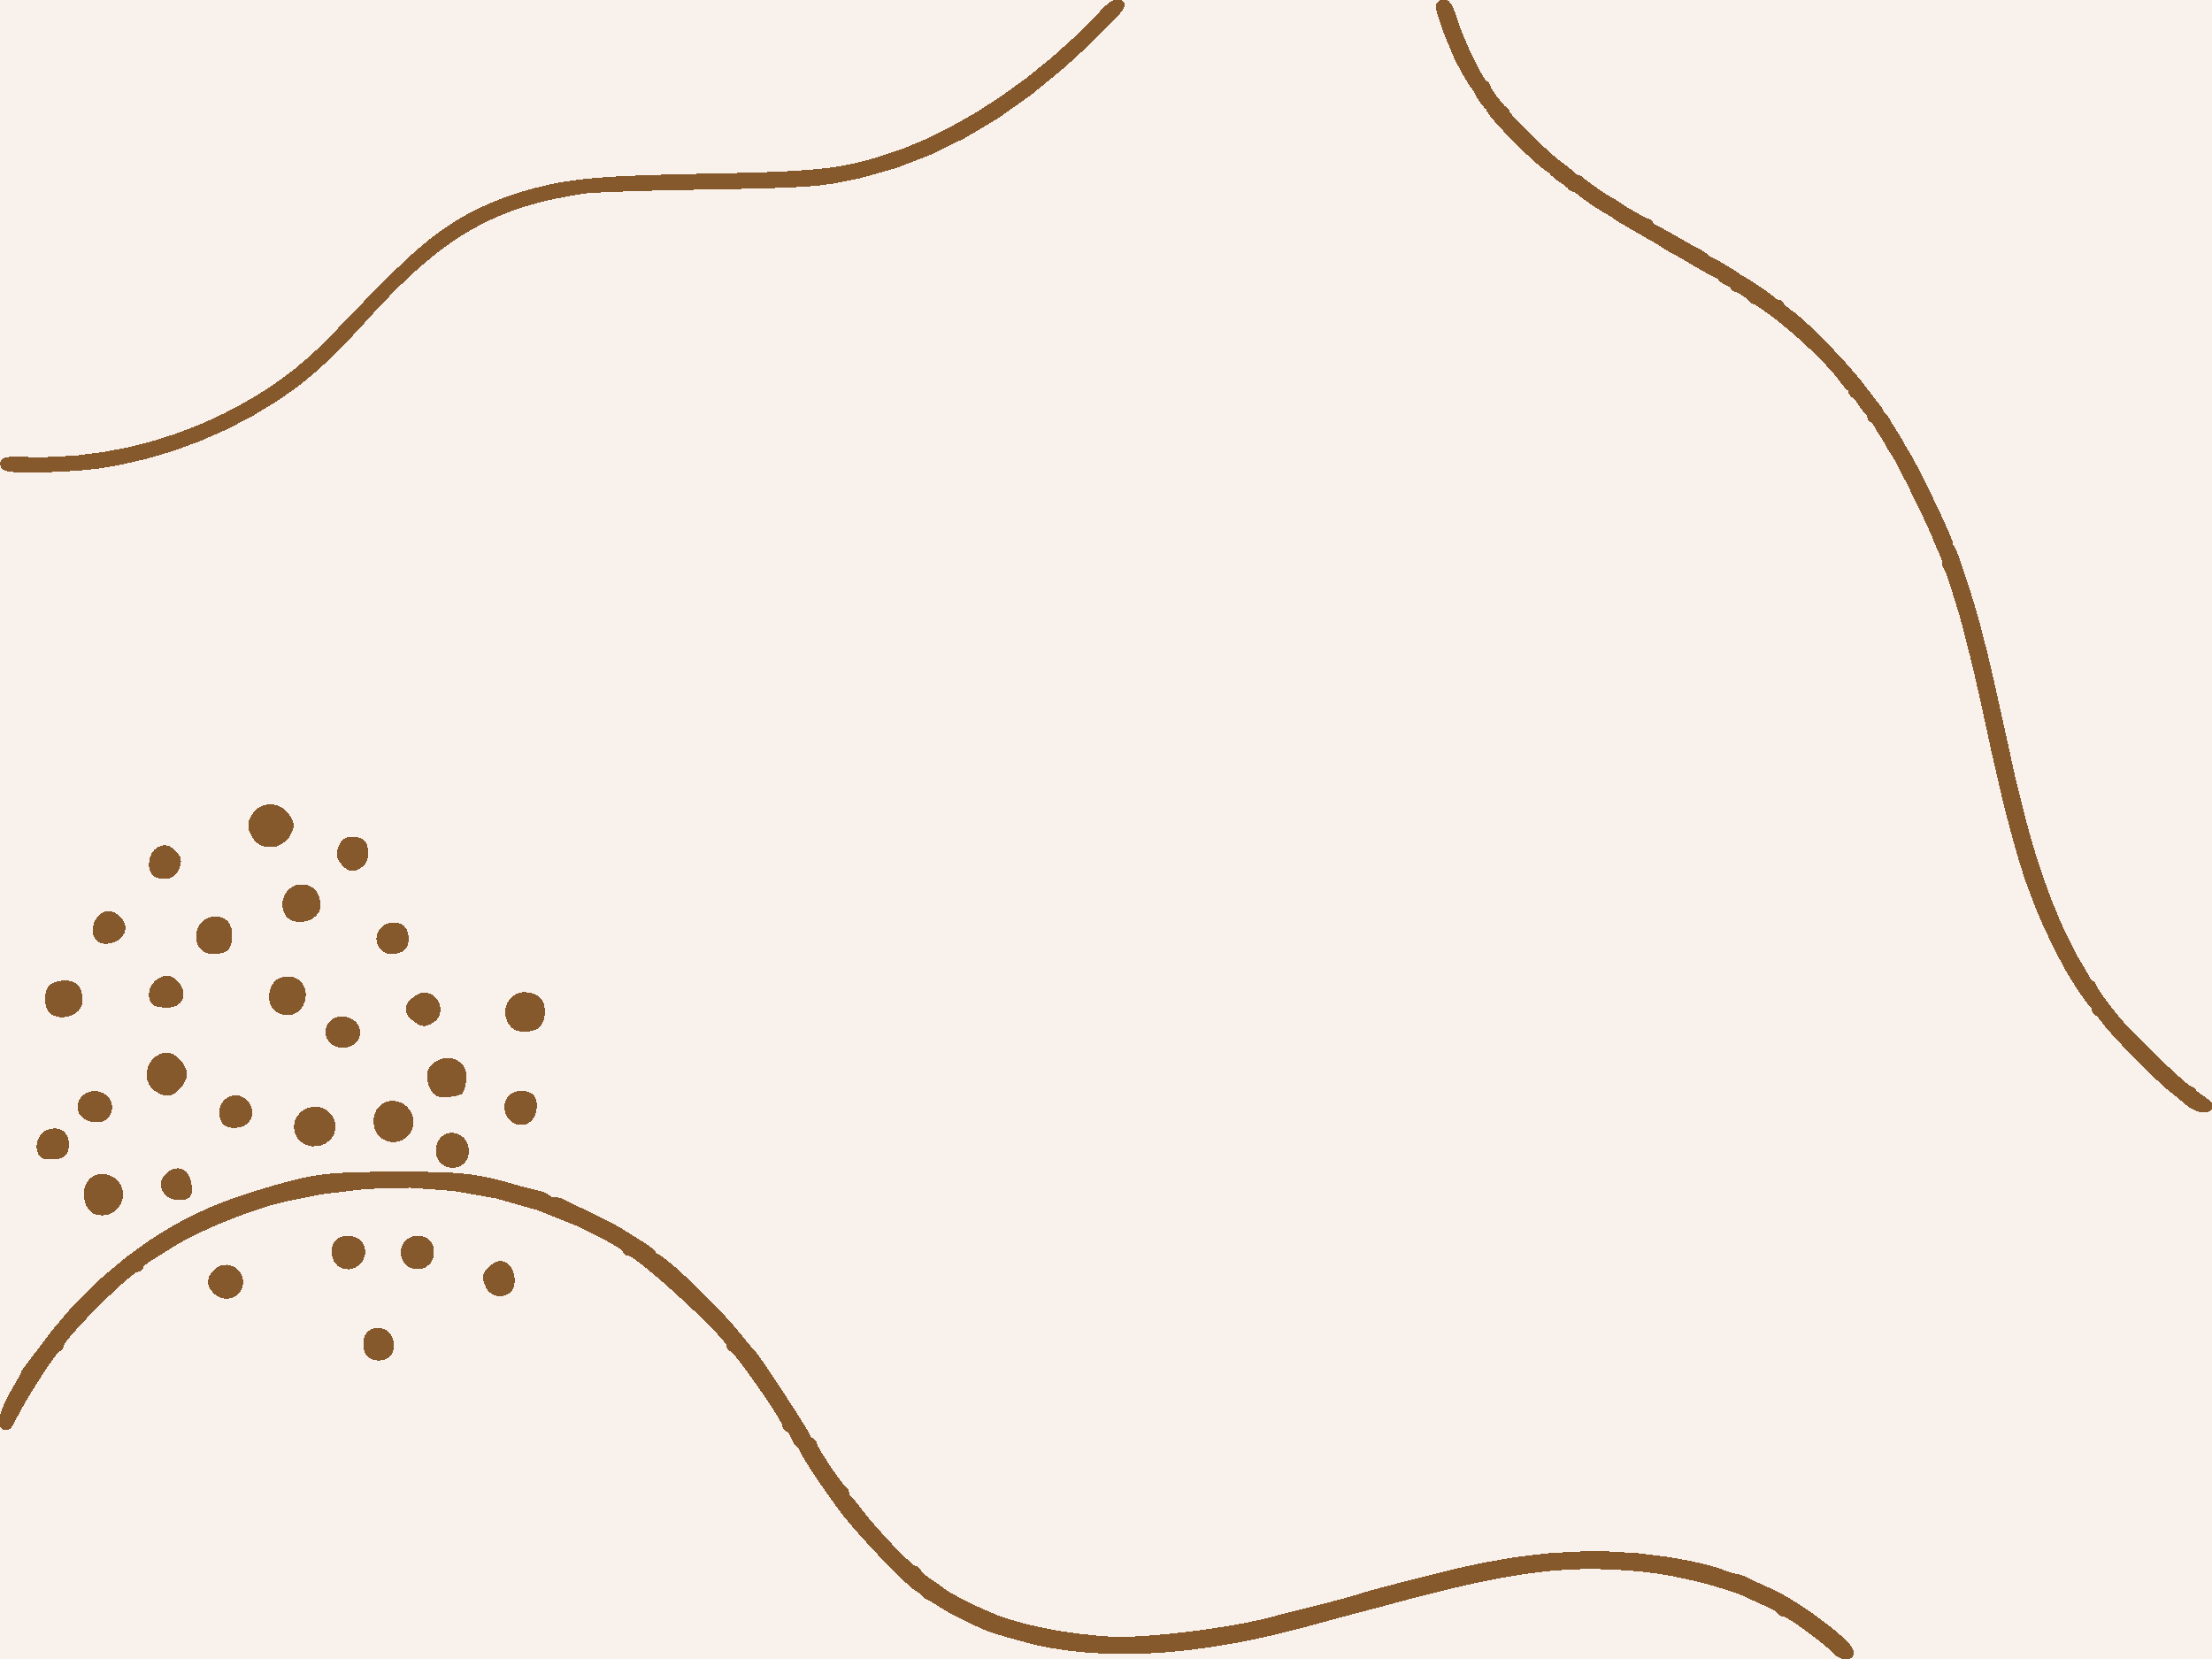
\includegraphics[width=\paperwidth,height=\paperheight]{images/assets/transition}}
\begin{frame}[noframenumbering]

\begin{center}
\Huge \textcolor{brown!70!black}{\textbf{Side-quests \\ and future works}}
\end{center}

\end{frame}}

%------------------------------------------------------------
\begin{frame}
\frametitle{Side quests}

\begin{exampleblock}{Anderson accelation method for self-consistence:}
\begin{itemize}
%\item \textcolor{ForestGreen!80!black}{\textbf{Check charge variance}}
\item \textcolor{ForestGreen!80!black}{\textbf{Fix convergence for larger $U$s} (notably in phase transitions)}
\item \textcolor{ForestGreen!80!black}{\textbf{Less iterations needed} (from $\sim 200$ to $\sim 20$)}
\end{itemize}
\end{exampleblock}
\pause

\setbeamercolor{itemize item}{fg=orange!95!black}
\begin{alertblock}{Other interesting models:}
\begin{itemize}
\item \textcolor{orange!95!black}{\textbf{Transversal modes} (role of the no. of transverse modes)}
\item \textcolor{orange!95!black}{\textbf{Closed loop} (possible oscilating pairing phase "soliton"?)}
\end{itemize}
\end{alertblock}
\pause

\setbeamercolor{itemize item}{fg=red!80!black}
\begin{block}{Complications to the models:}
\begin{itemize}
\item \textcolor{red!80!black}{\textbf{Disorder} (to solve Fermi $m_{0_\text{SC}}\neq m_{0_\text{SM}}$ mismatch in hybrid)}
\item \textcolor{red!80!black}{\textbf{Temperature influence} (tweak Schur solver in infinite case)}
\item \textcolor{red!80!black}{\textbf{Beyond local interactions} (allow for $U^\prime$ hoppings to NNN)}
\end{itemize}
\end{block}
\end{frame}

%------------------------------------------------------------
\begin{frame}
\frametitle{\underline{Future works:} Josephson junction loop}

\vspace*{-0.5cm}
\begin{center}
\begin{figure}
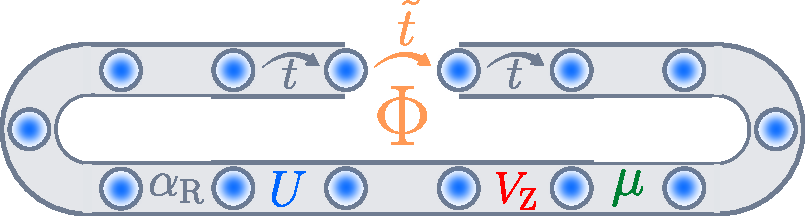
\includegraphics[scale=0.8]{images/model_ring}
\end{figure}
\end{center}

\begin{columns}
\column{3cm}
\begin{exampleblock}{Weak-link hop}
\vspace*{-4mm}
\begin{equation*}
\tilde{t}_{ij}=t_{ij}e^{-i\frac{e}{\hbar}\phi_{ij}}
\end{equation*}
\end{exampleblock}

\column{8cm}
\begin{alertblock}{Appropriate gauge}
\vspace*{-4mm}
\begin{equation*}
\phi_{ij}=\exp\left(-i\frac{e}{\hbar}\int_{\mathbf{r}_{i}}^{\mathbf{r}_{j}}d\mathbf{r}^{\prime}\cdot\mathbf{A}(\mathbf{r}^{\prime})\right)\textcolor{orange!95!black}{\longrightarrow}\ n\frac{\Phi}{\Phi_{0}}\delta_{i1}\delta_{jN}
\end{equation*}
\end{alertblock}
\end{columns}

\end{frame}

%------------------------------------------------------------
\begin{frame}
\frametitle{\underline{Future works:} Full-shell JJ}

\vspace*{2mm}
\begin{center}
\begin{figure}
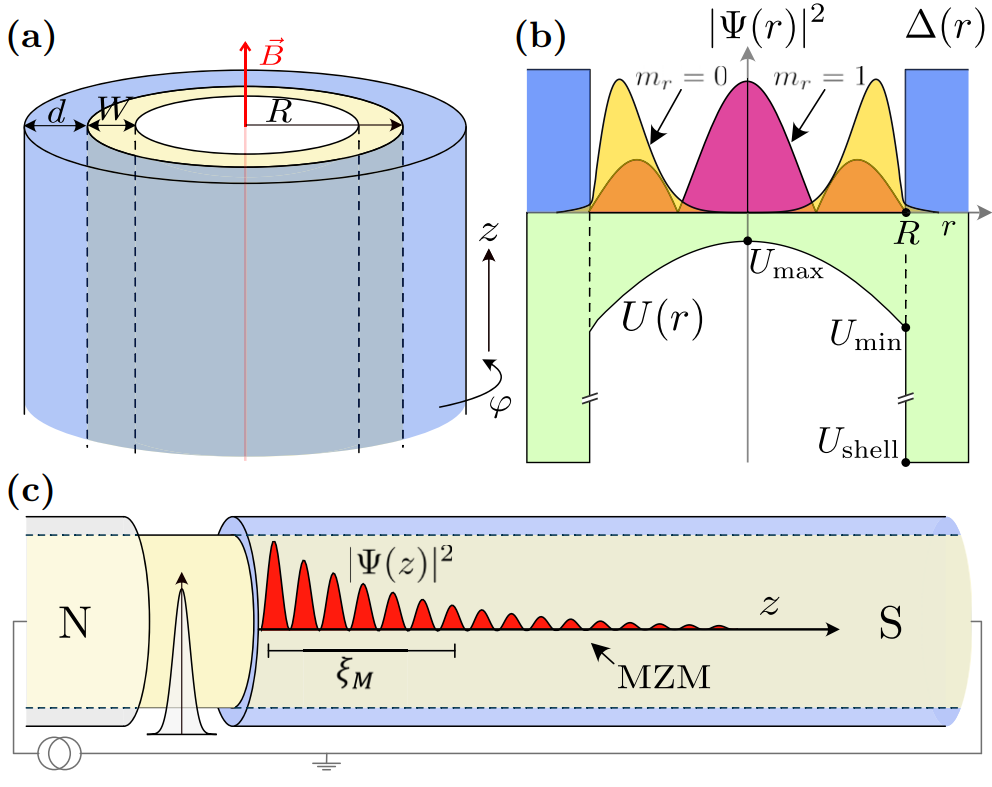
\includegraphics[scale=0.25]{images/fullshell}
\end{figure}
\end{center}

\textcolor{red!80!black}{*stolen from Physical Review B 109 (11), 115428}

\end{frame}

%------------------------------------------------------------
{\usebackgroundtemplate{

\includegraphics[width=\paperwidth,height=\paperheight]{images/assets/transition3}}
\begin{frame}[noframenumbering]

\vspace*{-30mm}
\begin{center}
\Huge \textcolor{brown!70!black}{\textbf{Thank you for listening!}} \\
\Huge \textcolor{brown!70!black}{\textbf{Any questions?}}
\end{center}

\end{frame}}

%------------------------------------------------------------
{\usebackgroundtemplate{
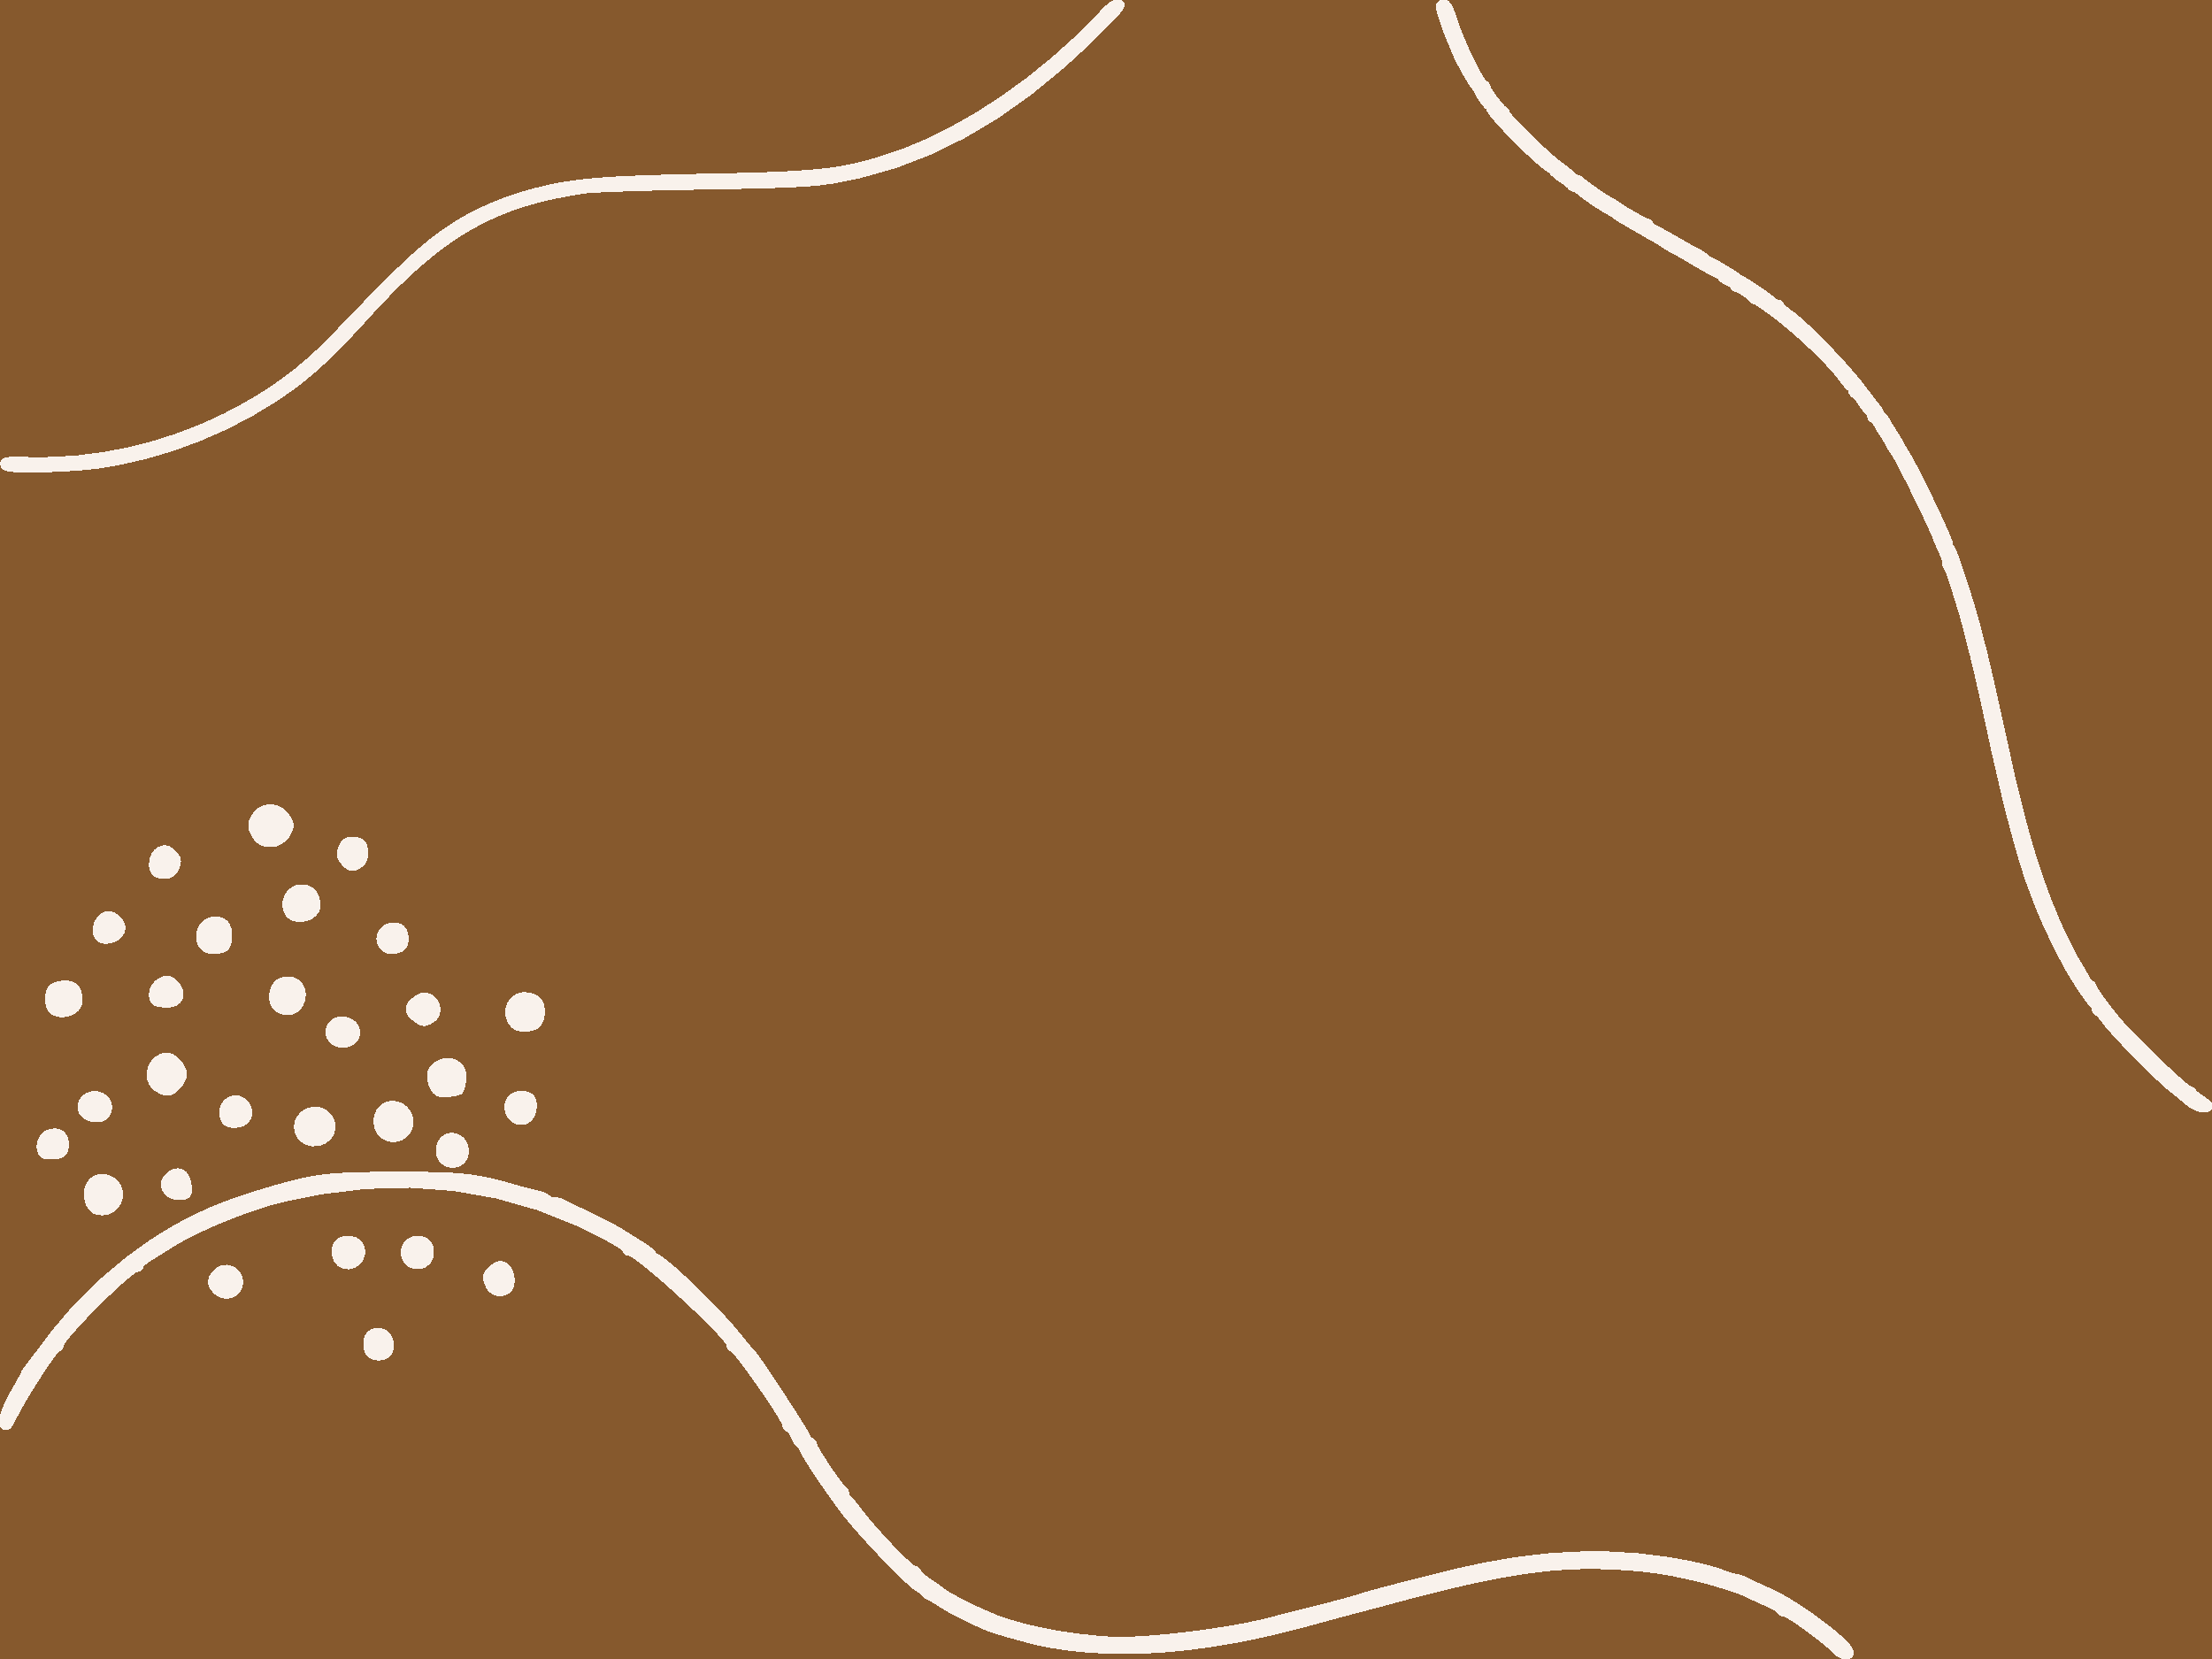
\includegraphics[width=\paperwidth,height=\paperheight]{images/assets/transition2}}
\begin{frame}[noframenumbering]

\begin{center}
\Huge \textcolor{brown!10!white}{\textbf{Appendix}}
\end{center}

\end{frame}}

%------------------------------------------------------------
{\usebackgroundtemplate{
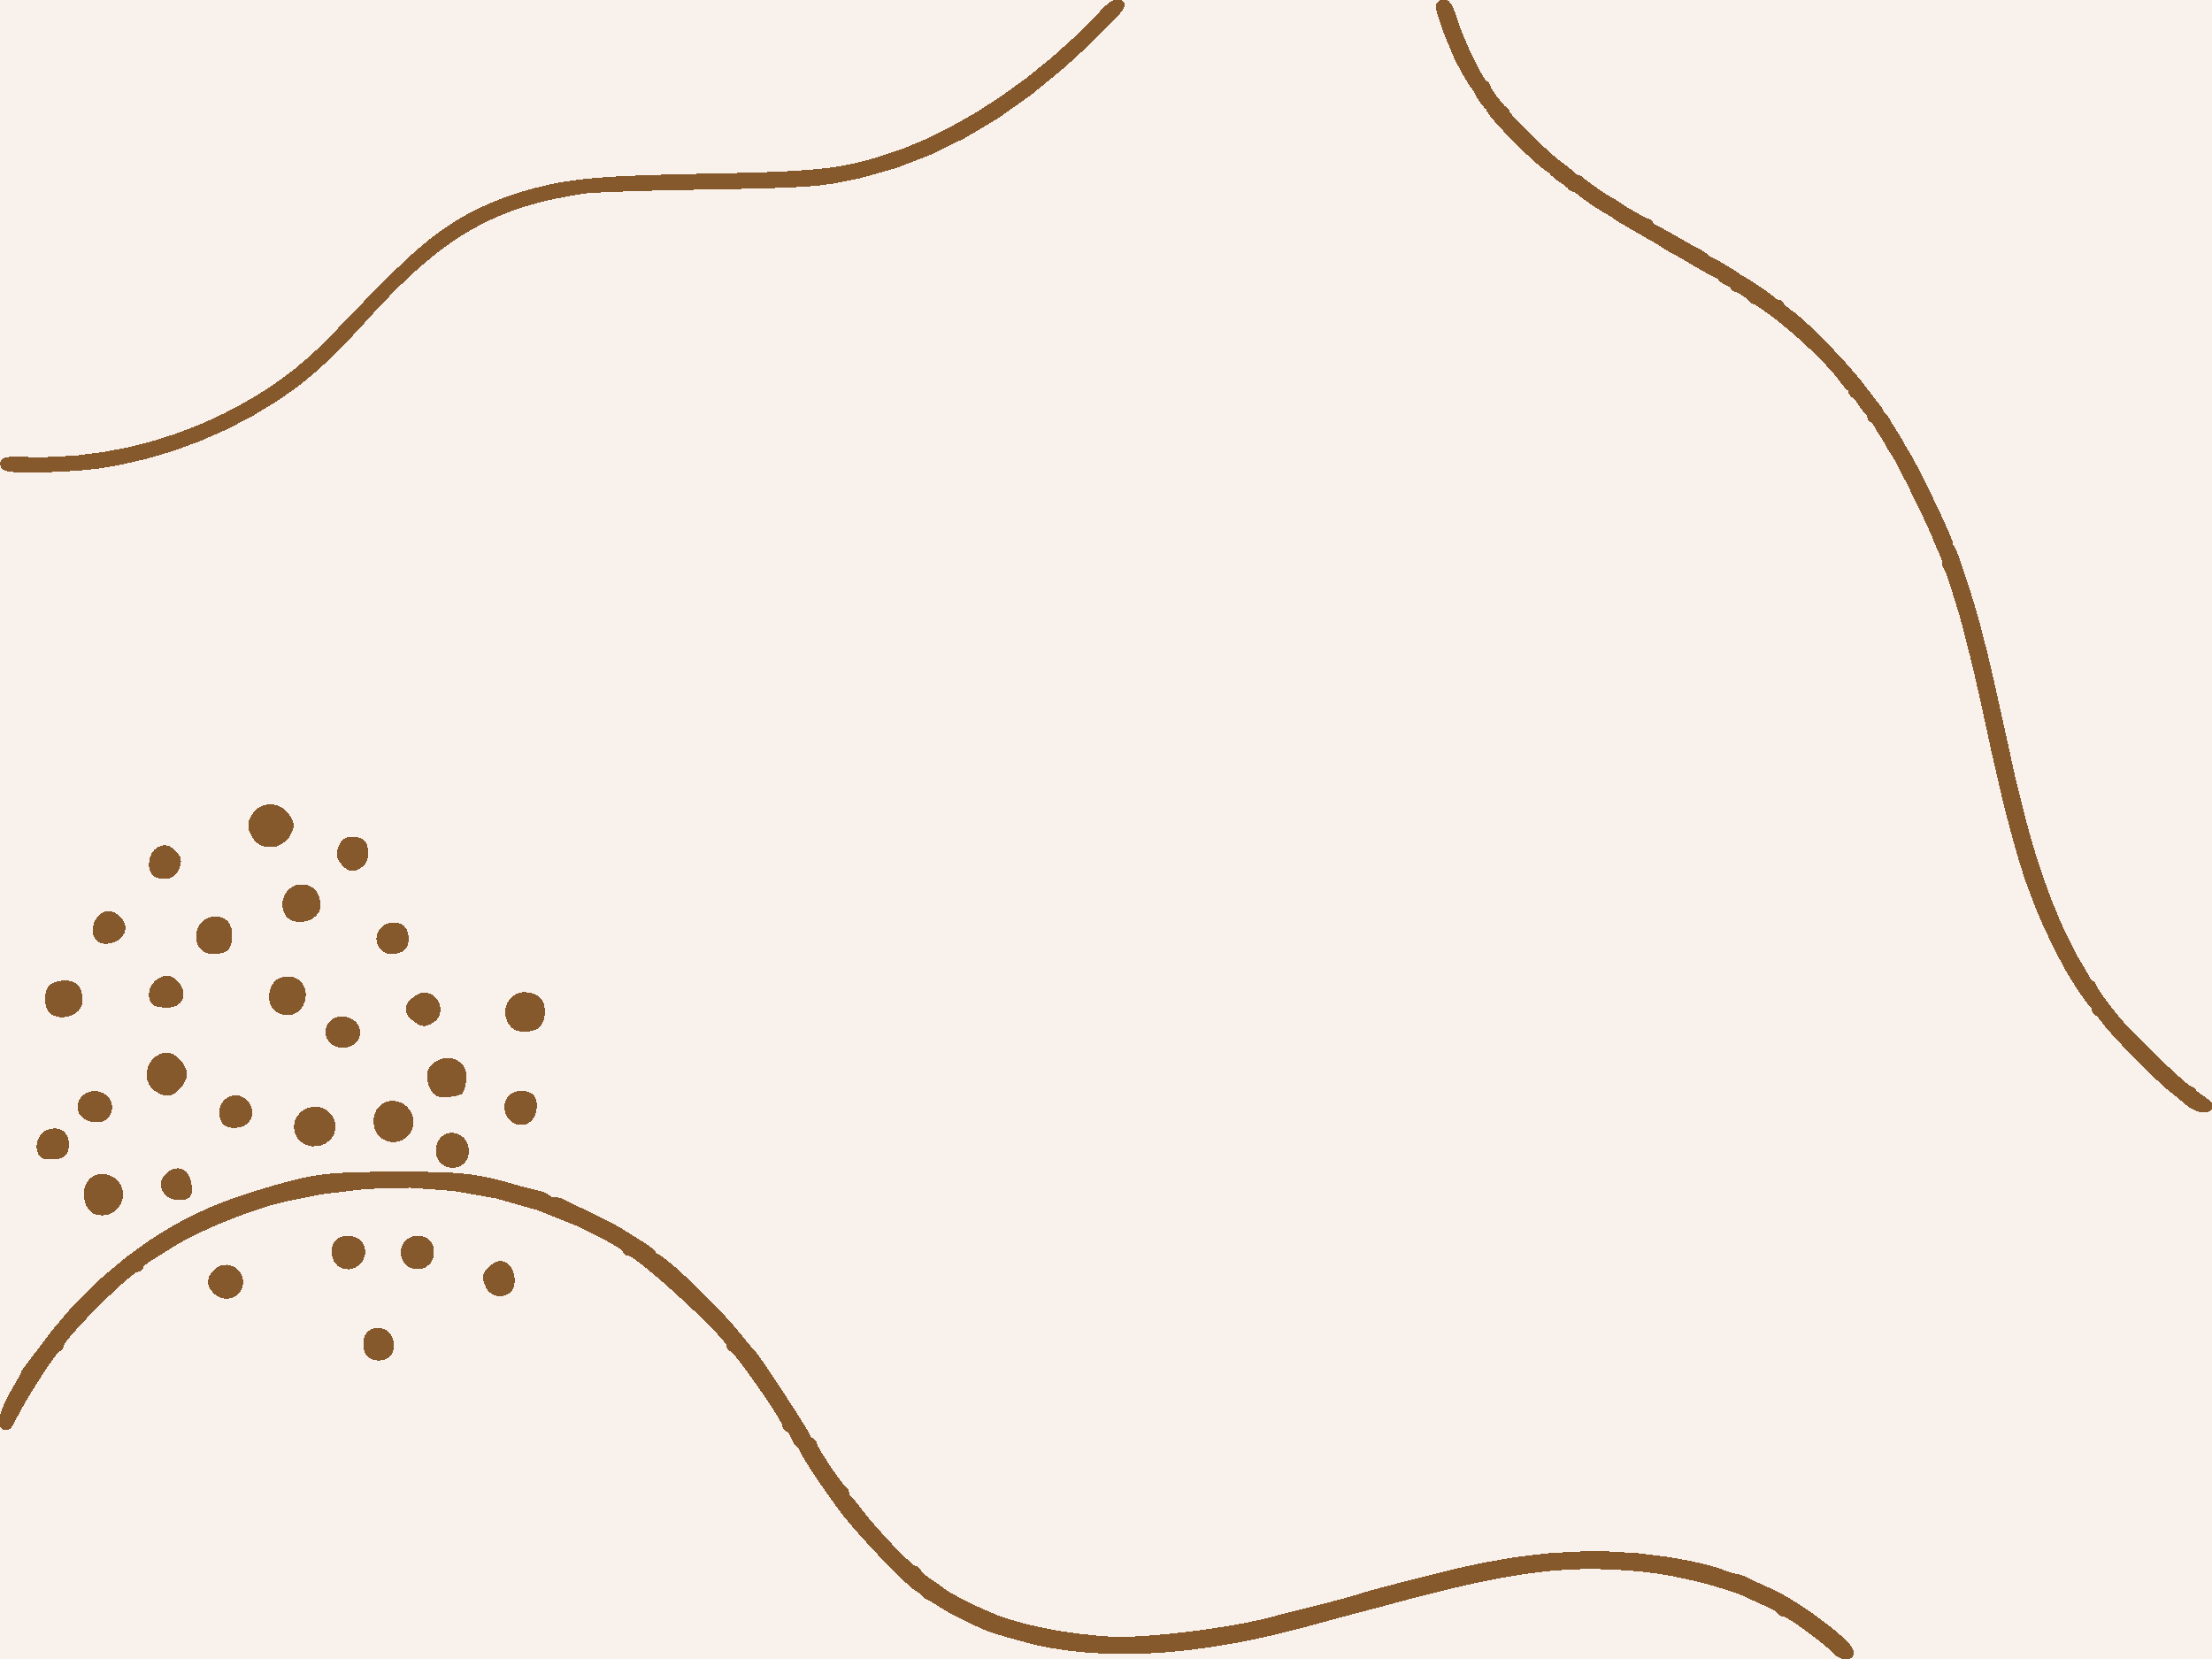
\includegraphics[width=\paperwidth,height=\paperheight]{images/assets/transition}}
\begin{frame}[noframenumbering]

\begin{center}
\Huge \textcolor{brown!70!black}{\textbf{Numerical details}}
\end{center}

\vspace*{1cm}
\begin{center}
\begin{figure}

\includegraphics[scale=0.3]{images/assets/Quanticajl}
\end{figure}
\end{center}

\end{frame}}

%------------------------------------------------------------
\begin{frame}[noframenumbering]
\frametitle{Numerical details: building the Hamiltonian}

\begin{center}
\begin{figure}
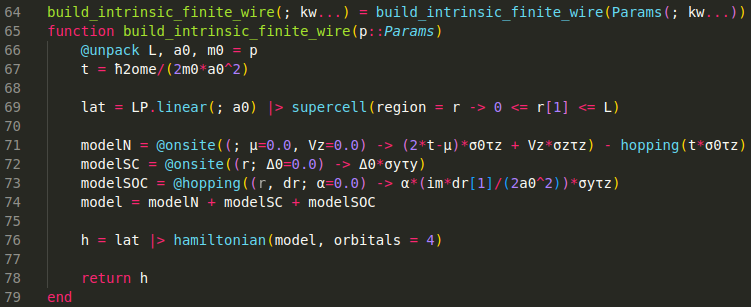
\includegraphics[scale=0.45]{images/quantica_buildwire}
\end{figure}
\end{center}

\end{frame}

%------------------------------------------------------------
\begin{frame}[noframenumbering]
\frametitle{Numerical details: self-consistent calculation}

\begin{center}
\begin{figure}
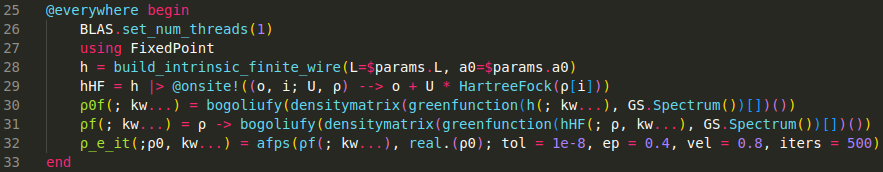
\includegraphics[scale=0.38]{images/quantica_selfconsistency}
\end{figure}
\end{center}

\begin{exampleblock}{Bogoliubov-DeGenes symmetries}
\vspace*{-4mm}
\begin{align*}
&\rho_{ab}^{\text{ee/hh}}=(\rho_{ba}^{\text{ee/hh}})^{*},\qquad\rho_{ab}^{\text{he}}=(\rho_{ba}^{\text{eh}})^{*},\\&\rho_{ab}^{\text{hh}}=-
\rho_{ba}^{\text{ee}}+\delta_{ab},\qquad\rho_{ba}^{\text{eh/he}}=-
\rho_{ab}^{\text{eh/he}}
\end{align*}
\end{exampleblock}

\begin{exampleblock}{For the \underline{infinite} case the Green's solver is instead \underline{Schur} factorization,}
\begin{equation*}
\rho_{dn}=\frac{1}{2\pi}\int_{-\pi}^{+\pi}d\phi f(H(\phi)-\mu I)e^{idn\phi}
\end{equation*}
\end{exampleblock}

\end{frame}

%------------------------------------------------------------
{\usebackgroundtemplate{
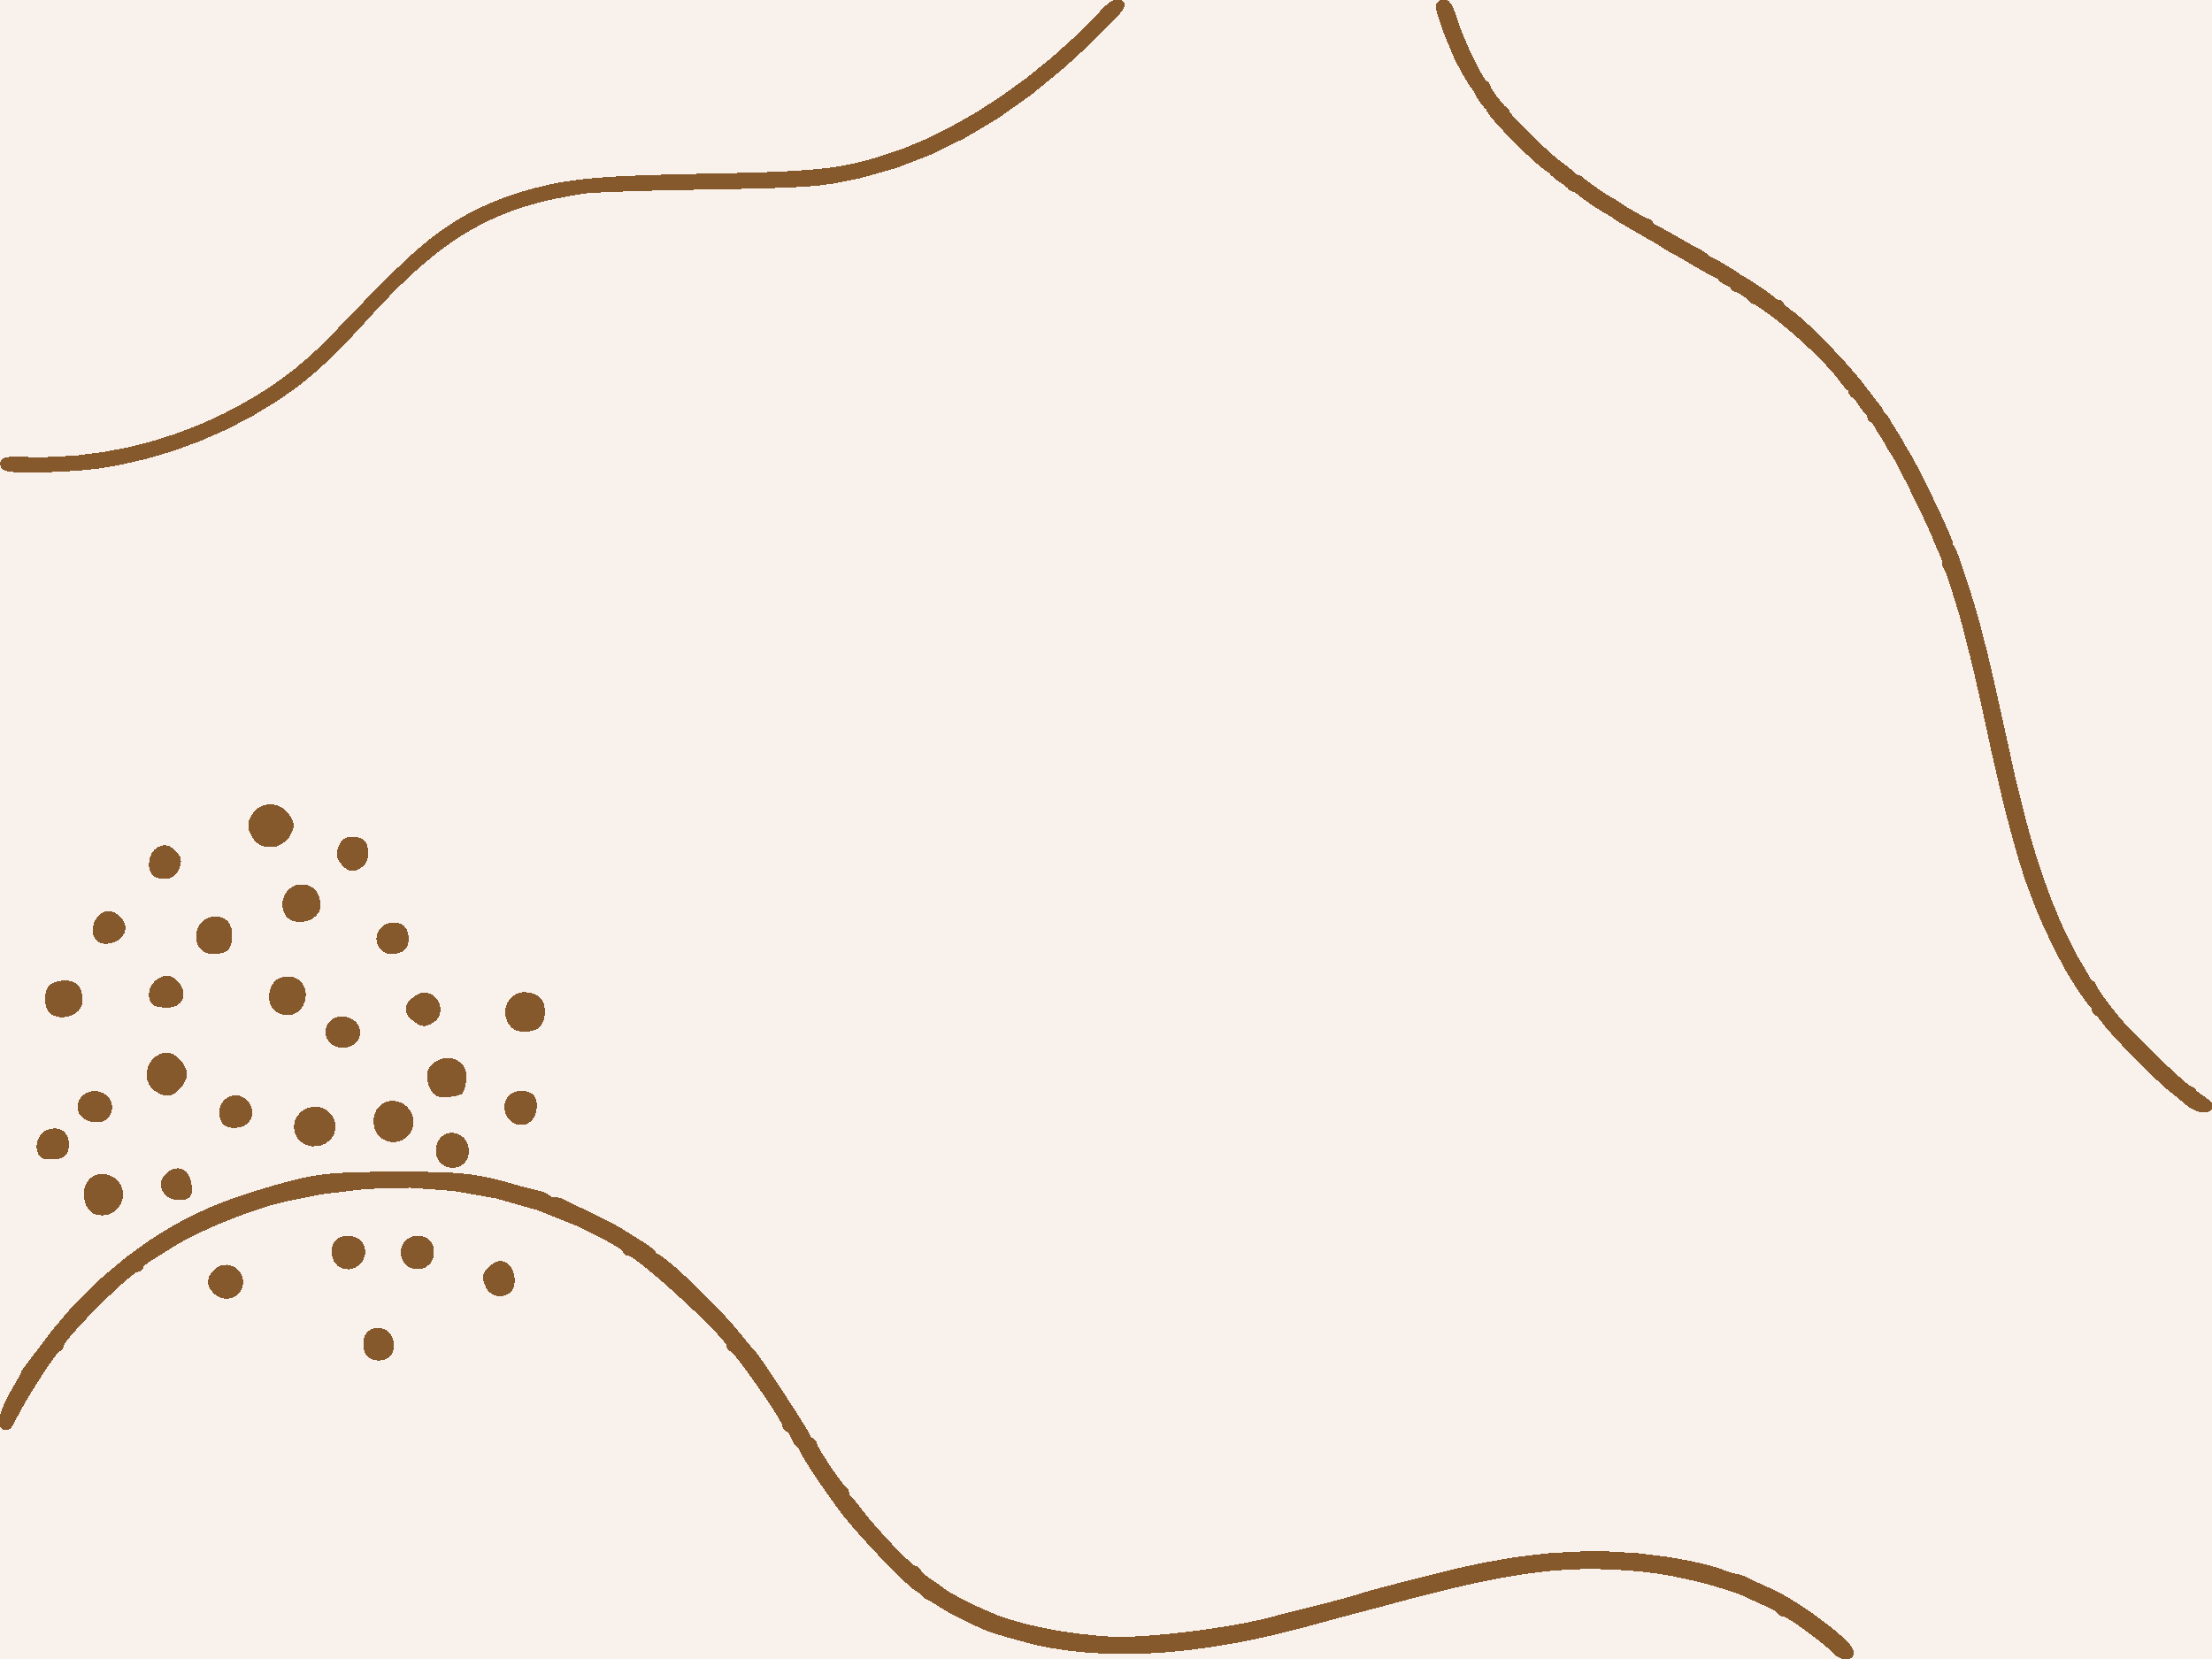
\includegraphics[width=\paperwidth,height=\paperheight]{images/assets/transition}}
\begin{frame}[noframenumbering]

\begin{center}
\Huge \textcolor{brown!70!black}{\textbf{Some other \\ extra details}}
\end{center}

\end{frame}}

%------------------------------------------------------------
\begin{frame}[noframenumbering]
\frametitle{Lutchyn's model with $\Delta_0\approx 0$}

\begin{center}
\begin{figure}
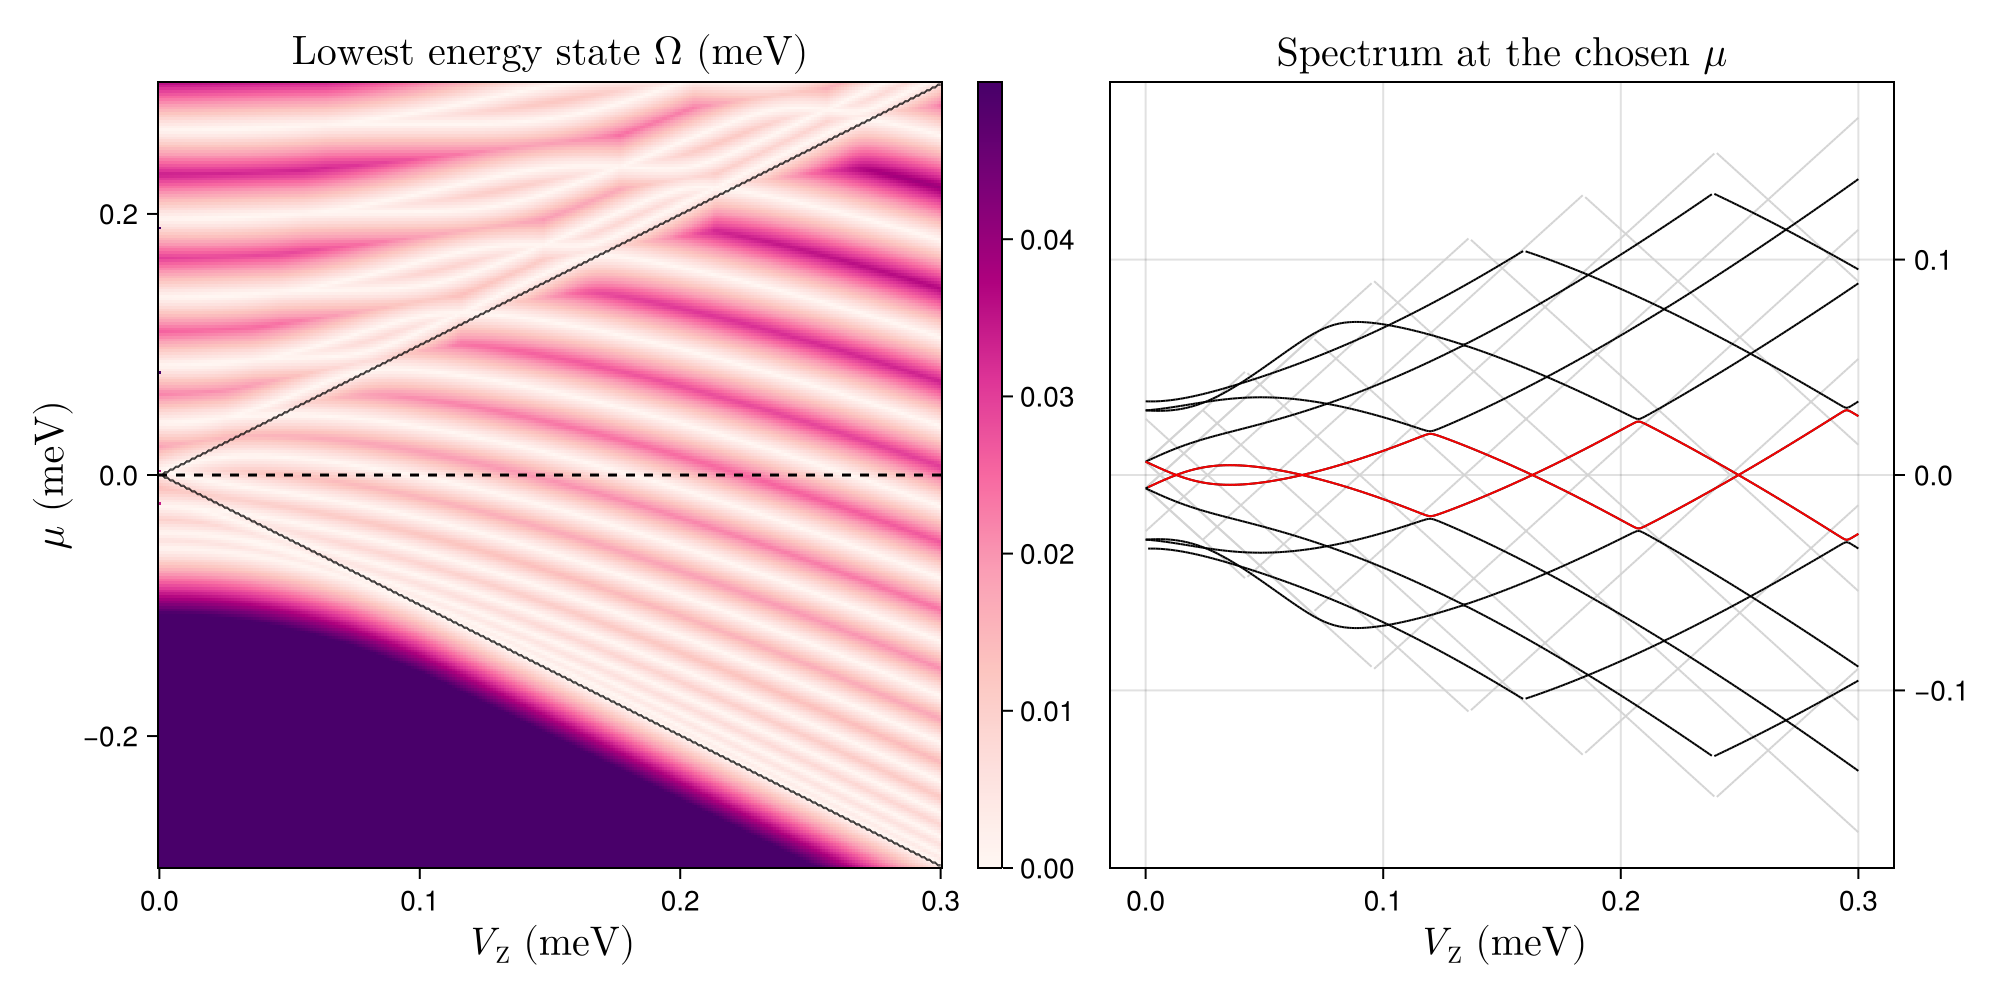
\includegraphics[scale=0.17]{images/lutchyn_D00_gap_spectrum}
\end{figure}
\end{center}
\end{frame}

%------------------------------------------------------------
\end{document}

